\documentclass[russian, hyperref={unicode}]{beamer}

\usetheme{Madrid}
\setbeamertemplate{footline}[frame number]
\setbeamertemplate{navigation symbols}{}
% \setbeameroption{show only notes}
\setbeamerfont{note page}{size=\footnotesize}

\usepackage[T2A]{fontenc}
\usepackage{lmodern}
\usepackage[utf8x]{inputenc}
\usepackage[english, russian]{babel}
\usepackage{graphicx}

\usepackage{algpseudocode}
\algtext*{EndWhile}     % Remove "end while" text
\algtext*{EndFor}       % Remove "end for" text
\algtext*{EndFunction}  % Remove "end function" text
\algtext*{EndIf}        % Remove "end if" text

\graphicspath{ {../Images/} }

% workaroung warning
\let\Tiny=\tiny

\title{Построение семейств оптимальных маршрутов на морских картах}
\author{Иван Громаковский \\
Научный руководитель: А. С. Ковалев}
\institute{Санкт-Петербургский национальный исследовательский университет \\ информационных технологий, механики и оптики}
\date{}

\begin{document}

\section{Введение}

\frame{\titlepage}
\note{Здравствуйте!}

\subsection{Неформальная постановка}

\begin{frame}{Описание задачи}
    \only<1-3> {
        \begin{itemize}
            \item Имеется морская навигационная карта
            \item Требуется предоставить возможность найти как можно
              больше непохожих маршрутов между двумя точками
            \item Задача поддержки принятия решения ⇒ real time
            \item<2-3> \alert{Не требуется находить кратчайший маршрут, однако
              маршруты должны быть не сильно длиннее кратчайшего}
        \end{itemize}
        \uncover<3> {
            \begin{columns}
                \column{.5\textwidth}
                    \begin{figure}
                        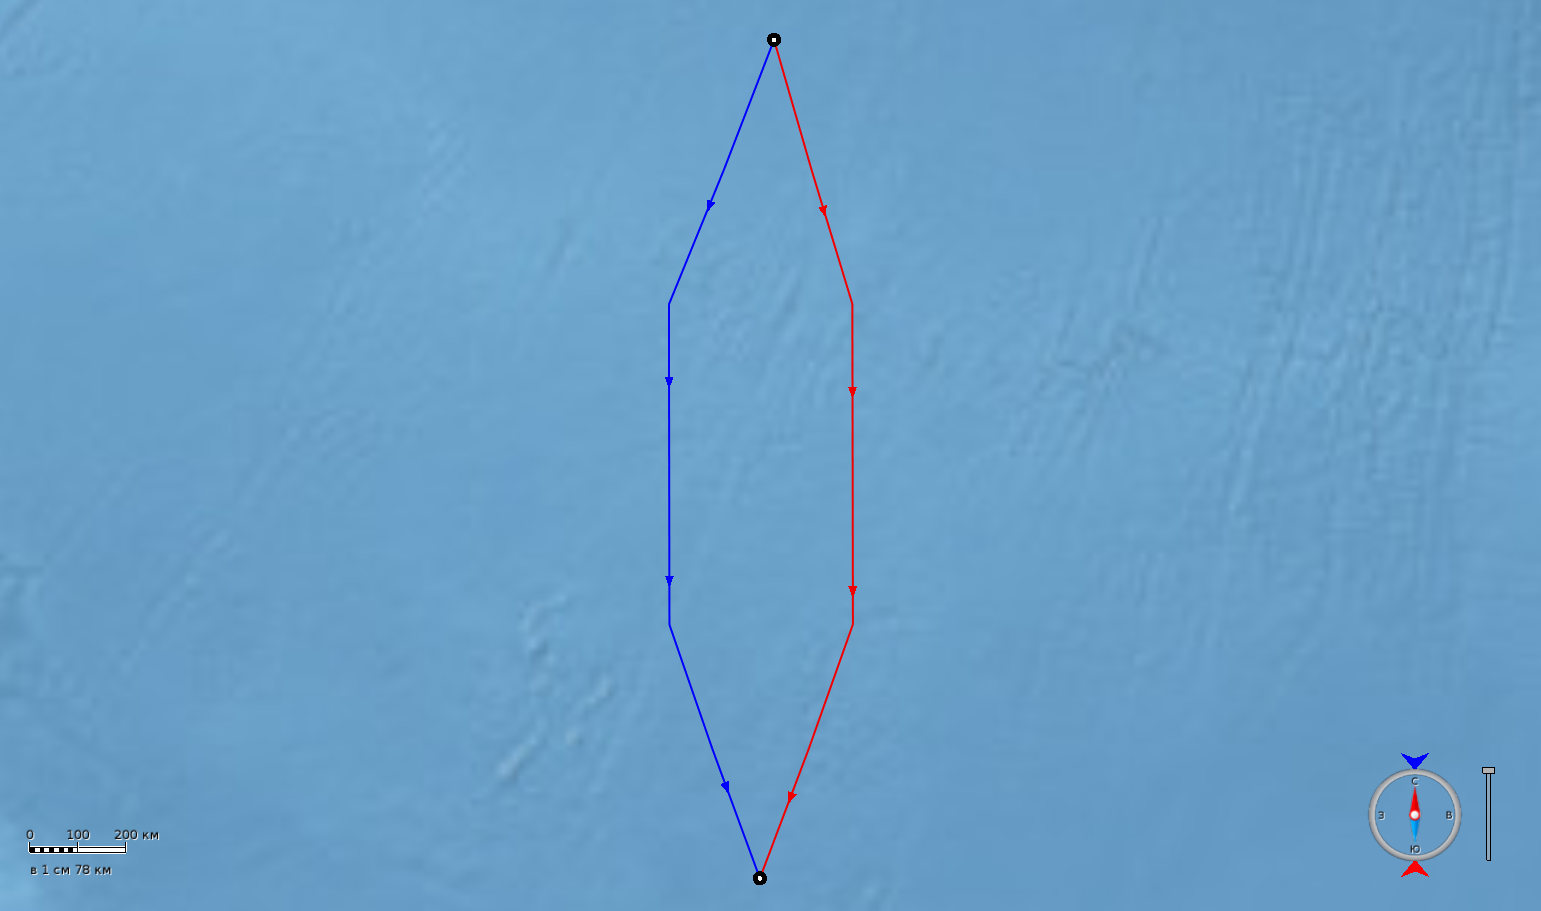
\includegraphics[width=\textwidth]{Introduction/similar}
                        
                        Похожие маршруты
                    \end{figure}
                \column{.5\textwidth}
                    \begin{figure}
                        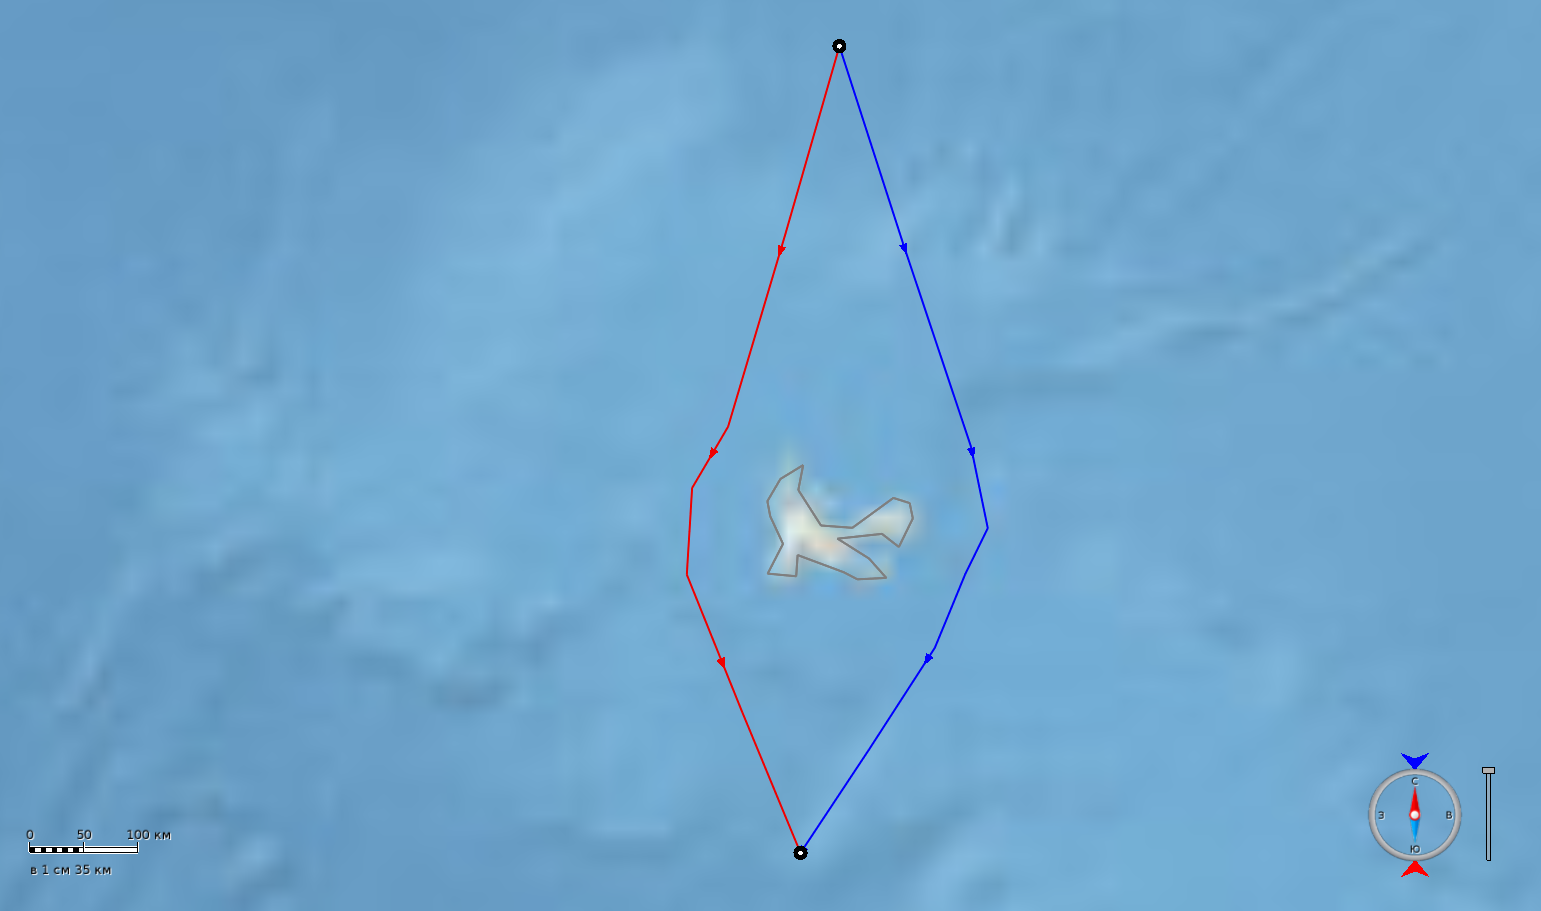
\includegraphics[width=\textwidth]{Introduction/dissimilar}

                        Непохожие маршруты
                    \end{figure}
            \end{columns}
        }
    }
    \only<4> {
        \begin{figure}
            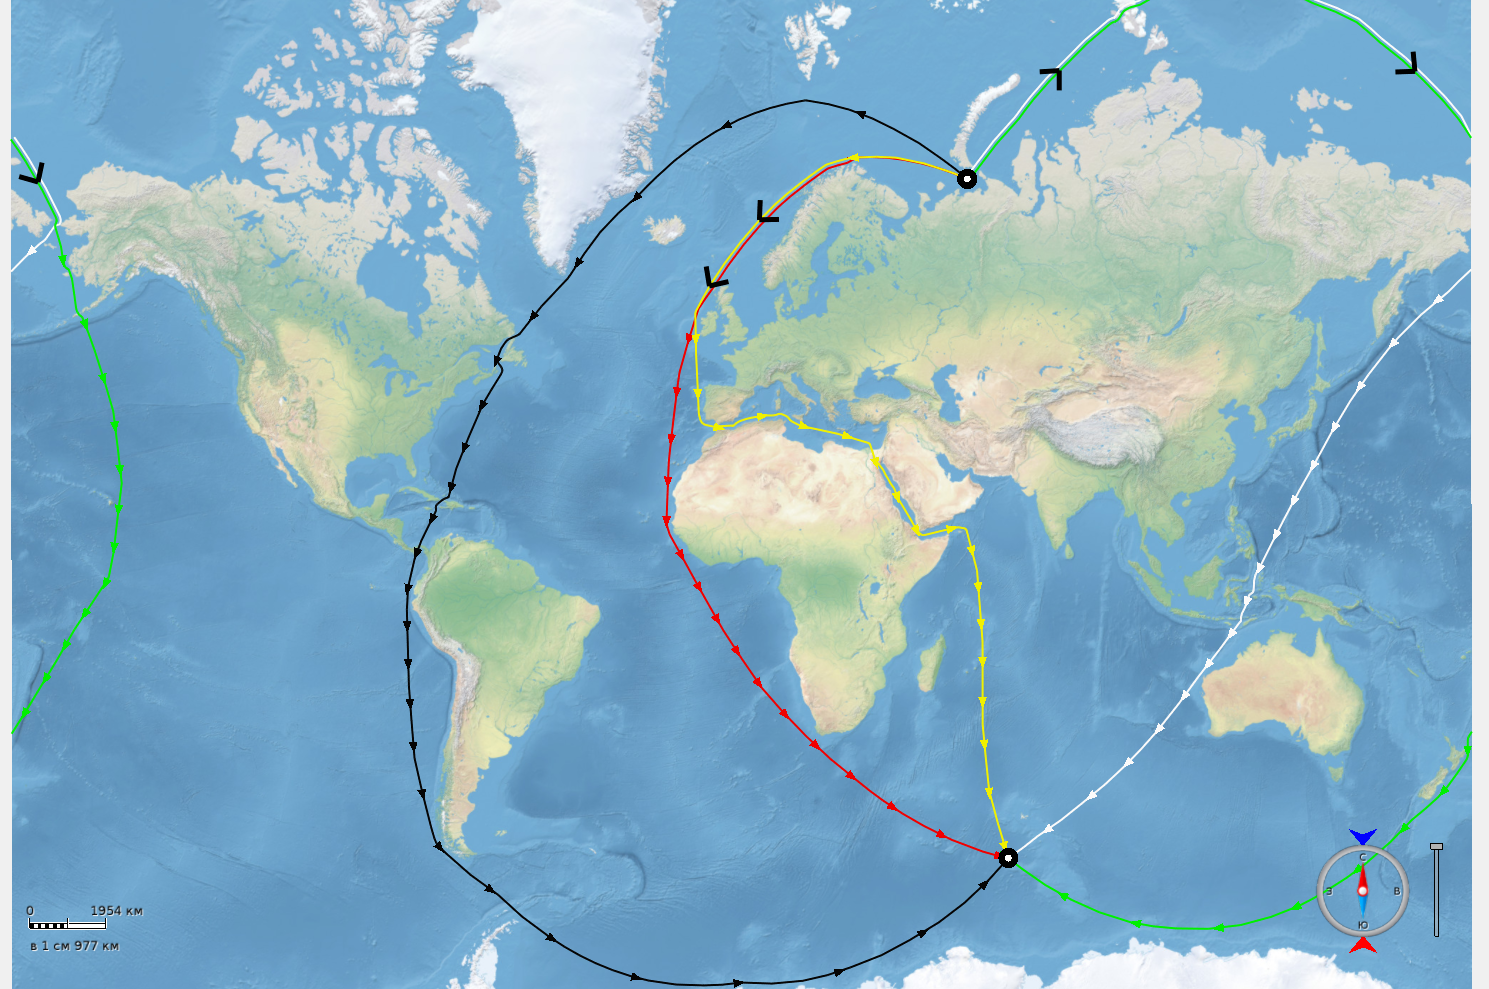
\includegraphics[width=.95\textwidth]{Introduction/my-good}

            Пример
        \end{figure}
    }
\end{frame}
\note {
Начну с неформального описания задачи. Имеется морская навигационная
карта, требуется предоставить пользователю возможность найти как можно
больше непохожих маршрутов по воде. При этом само по себе решение
задачи не является конечным результатом, а лишь поддержкой принятия
решения. Само решение принимается пользователем в голове, поэтому
основной принцип подобных задач в том, что они должны решаться в
режиме реального времени, чтобы не сбивать пользователя с мыслей.

Важно отметить, что в задаче не подразумевается поиск кратчайшего
маршрута. Суть задачи в предложении альтернативных путей, которые
потенциально могли бы быть выбраны.

На картинках проиллюстрировано понятие непохожести маршрутов. Для
простоты взят небольшой остров, но вместо него мог бы быть и материк.
}

\begin{frame}{Актуальность задачи}
    Проблемы поиска единственного маршрута:
    \begin{itemize}
        \item критерии оптимальности не всегда очевидны и формализуемы
        \item ненадёжность
    \end{itemize}
    \uncover<2>{Неизвестны алгоритмы multipath planning на воде}
\end{frame}
\note {
Поясню, зачем это нужно.

Задача поиска кратчайшего маршрута при наличии полигональных
препятствий хорошо известна и исследована, однако при таком подходе
возникают следующие проблемы:
\begin{itemize}
\item Кратчайший путь (по какой-либо метрике) не всегда оптимален, а
реальные критерии оптимальности могут быть не очевидны и трудно
формализуемы.

\item Если по каким-то причинам проплыть по кратчайшему маршруту не
представляется возможным (например, проходят учения), то возникает
проблема, потому что нет альтернатив.
\end{itemize}

При этом неизвестны алгоритмы multipath planning (то есть, поиска
нескольких маршрутов), которые бы хорошо работали на воде.
}
        
\subsection{Обзор сделанного}

\begin{frame}{Существующие алгоритмы}
    \only<1> {
        Известные алгоритмы multipath planning:
        \begin{itemize}
            \item разрабатывались для других целей
            \item не учитывают реальное физическое расположение
              вершин в графе
            \item строят очень похожие маршруты на морских картах
        \end{itemize}
    }
    \only<2> {
        \begin{figure}
            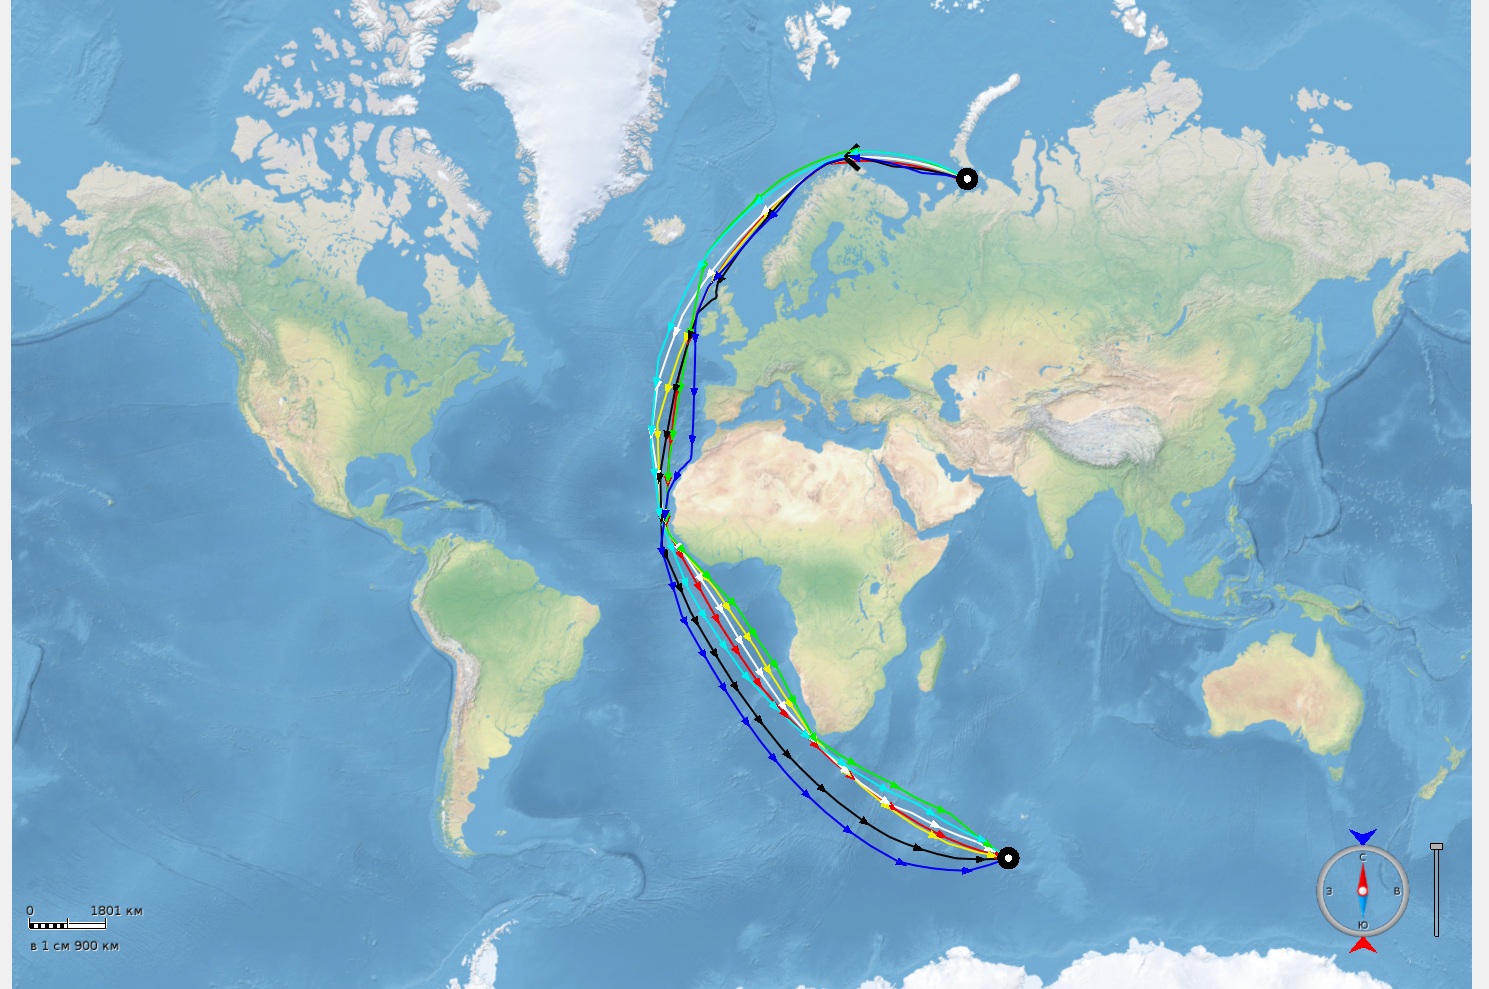
\includegraphics[width=.95\textwidth]{Introduction/existing-bad}

            Lim, Kim, 2005
        \end{figure}
    }
\end{frame}
\note {
Что касается известных алгоритмов поиска нескольких путей в графе, то
им присущи следующие проблемы:
\begin{itemize}
\item
Разрабатывались для других целей: например, поиск маршрутов по дорогам
или поиск маршрутов на общественном транспорте.
\item
Эти алгоритмы в большинстве своём оперируют абстрактными графами, не
привязанными к конкретным координатам в мире.
\item
Как следствие, попытка применить эти алгоритмы к данной задаче
приводит к похожим маршрутам.
\end{itemize}

Пример: видно, что маршруты почти не имеют общих рёбер, однако,
неформально говоря, они очень похожи. 
}

\subsection{Формальная постановка}

\begin{frame}{Формальная постановка задачи}
    Дано: множество полигональных препятствий, начальная (S) и конечная (D) точки.

    Найти: множество путей, соединяющих точки S и D и удовлетворяющих требованиям:
    \begin{itemize}
        \item отношение длины пути к длине кратчайшего пути
          ограничено сверху константой
        \item для любых двух путей выполнен критерий непохожести
    \end{itemize}

    Время выполнения запроса: меньше секунды
\end{frame}
\note {
Теперь сформулируем задачу формально.

Более-менее всё можно просто зачитать. Про критерий непохожести будет
сказано на следующем слайде. Поскольку требуется искать маршруты в
реальном времени, потребуем не больше секунды на запрос.
}

\begin{frame}[t]{Метрики на маршрутах}
    \only<1> {
        \begin{figure}[c]
            \begin{equation*}
                \rho_1 (P, Q) = \max(\max_{u \in P} \min_{v \in Q} \rho_g(u,
                v), \max_{u \in Q} \min_{v \in P} \rho_g(u, v))
            \end{equation*}
            \begin{equation*}
                \rho_2 (P, Q) = \max(\max_{u \in P} \frac{\min\limits_{v \in Q_u}
                \rho_g(u, v)}{\min\limits_{v \in Q_u} \rho_r(u, v)}, \max\limits_{u \in Q} \frac{\min\limits_{v \in P_u}
                \rho_g(u, v)}{\min\limits_{v \in P_u} \rho_r(u, v)})
            \end{equation*}
            \begin{equation*}
                Q_u = \{ v \in Q : \rho_r(u, v) > \varepsilon \cdot len(Q) \}
            \end{equation*}
        \end{figure}
    }
    \only<2> {
        \begin{figure}
            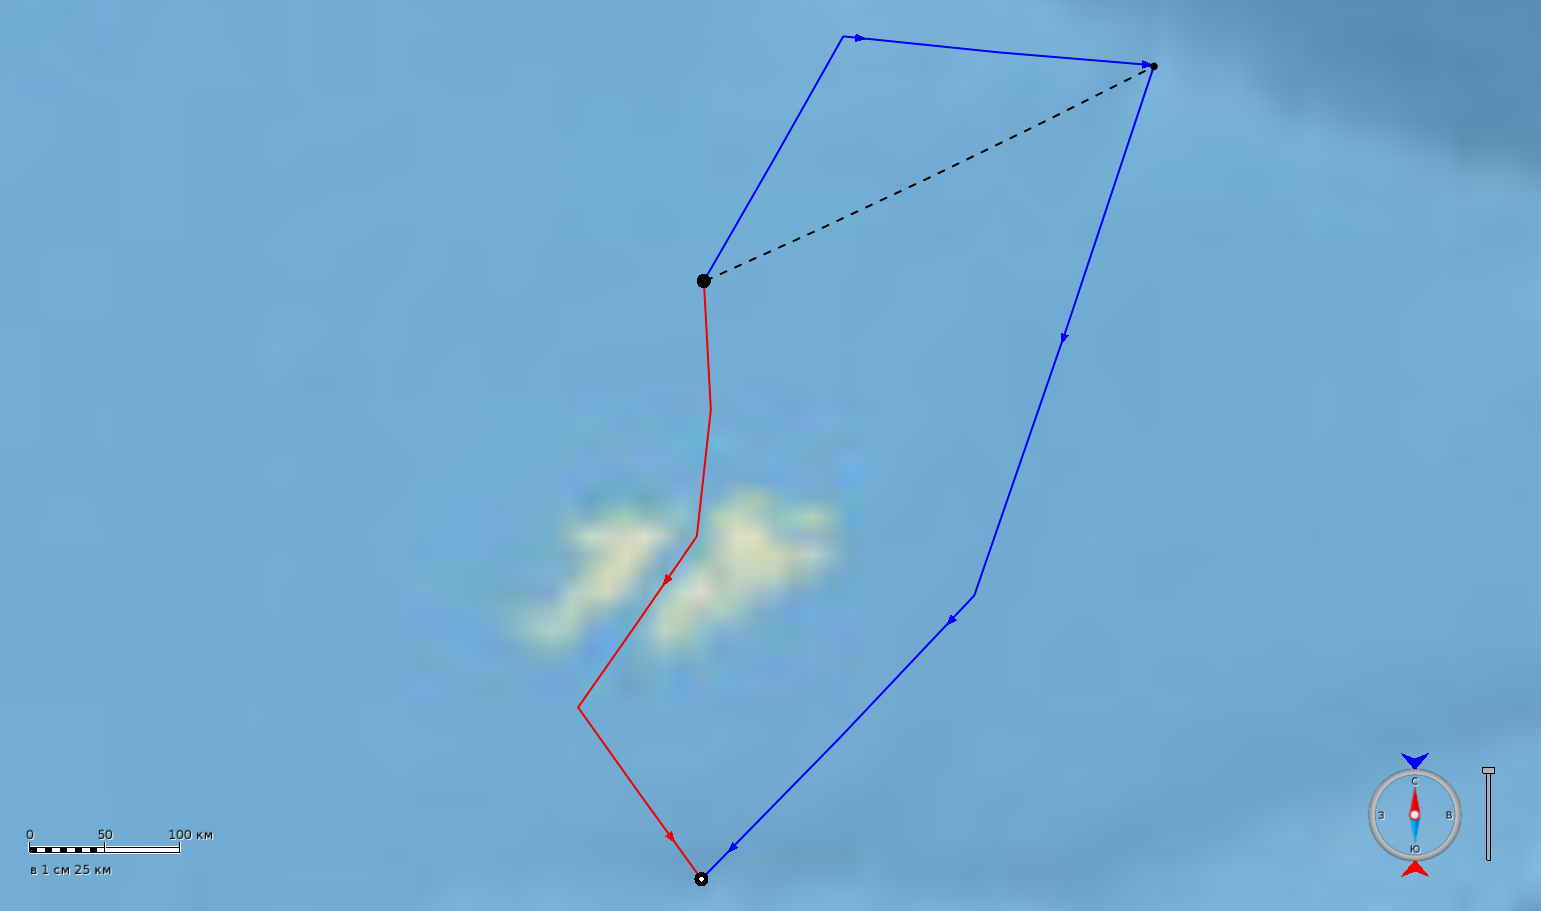
\includegraphics[width=.9\textwidth]{Solution/metrics/1-dissimilar}
            
            $\frac{\rho_1}{l_{min}} = \frac{339}{435} = 0.78$
        \end{figure}
    }
    \only<3> {
        \begin{figure}
            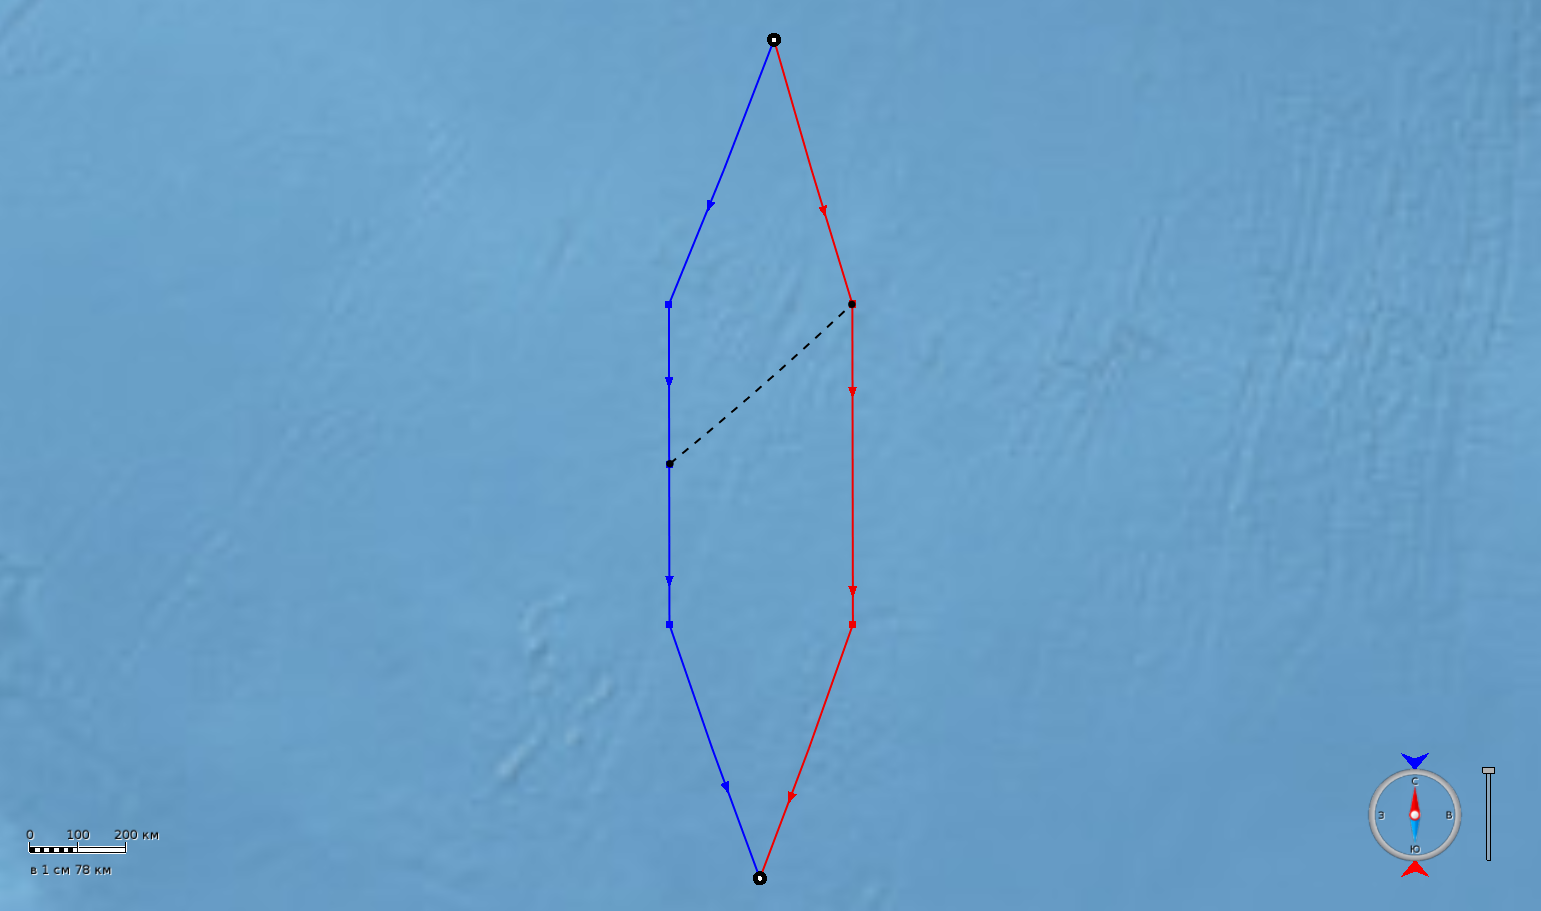
\includegraphics[width=.9\textwidth]{Solution/metrics/1-uncertain-2-similar}
            
            $\frac{\rho_1}{l_{min}} = \frac{502}{1704} = 0.29$

            $\rho_2 = 1$
        \end{figure}
    }
    \only<4> {
        \begin{figure}
            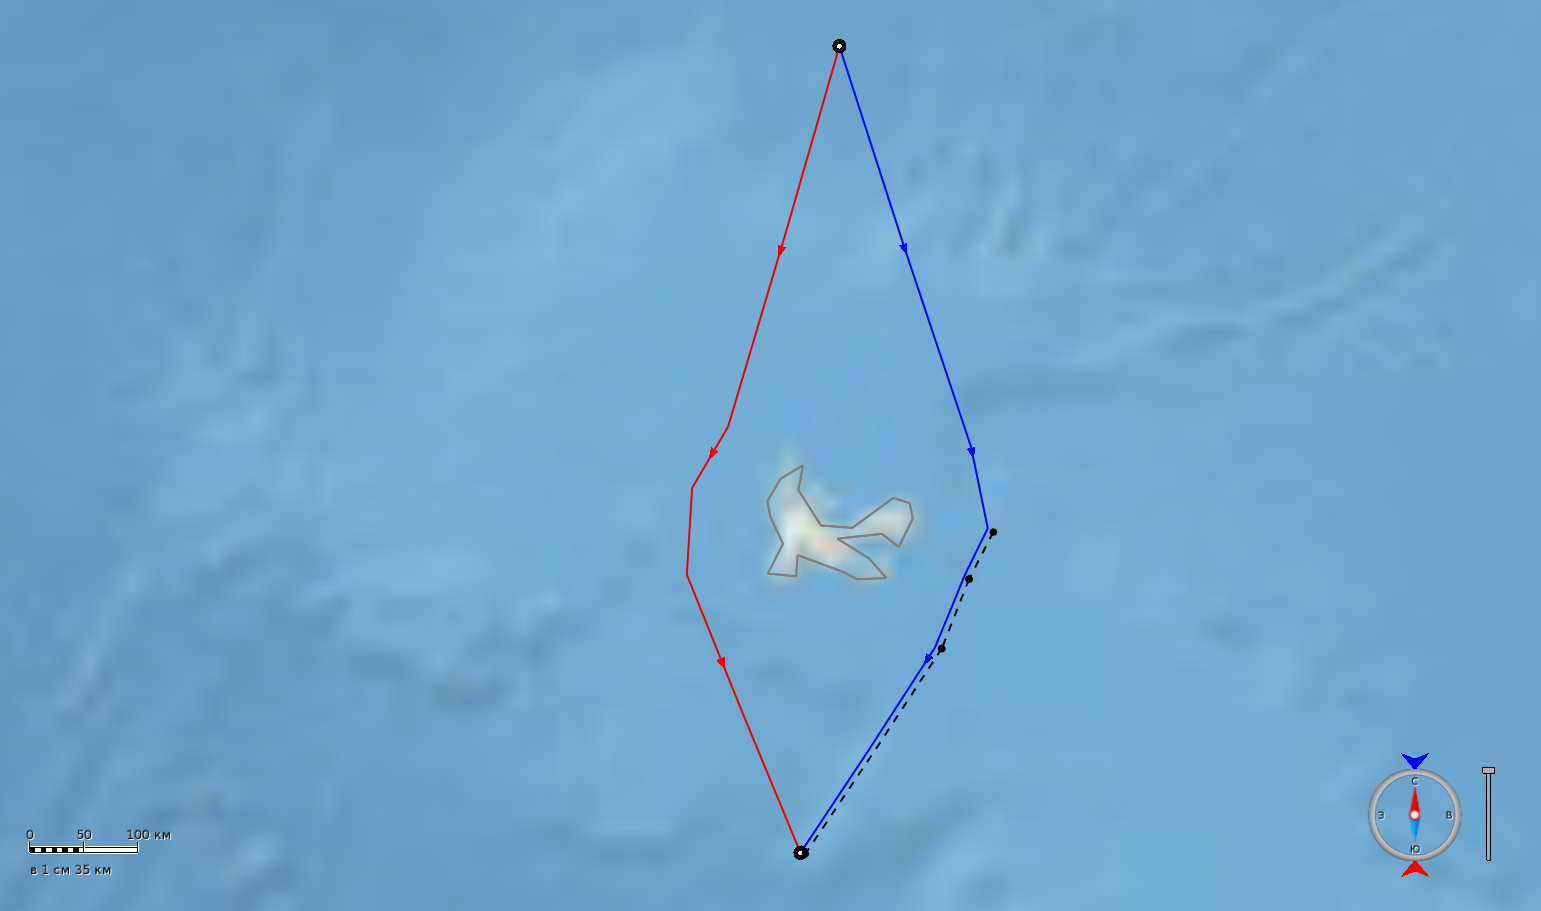
\includegraphics[width=.9\textwidth]{Solution/metrics/1-uncertain-2-dissimilar-gclosest}
            
            $\frac{\rho_1}{l_{min}} = \frac{307}{814} = 0.38$
        \end{figure}
    }
    \only<5> {
        \begin{figure}
            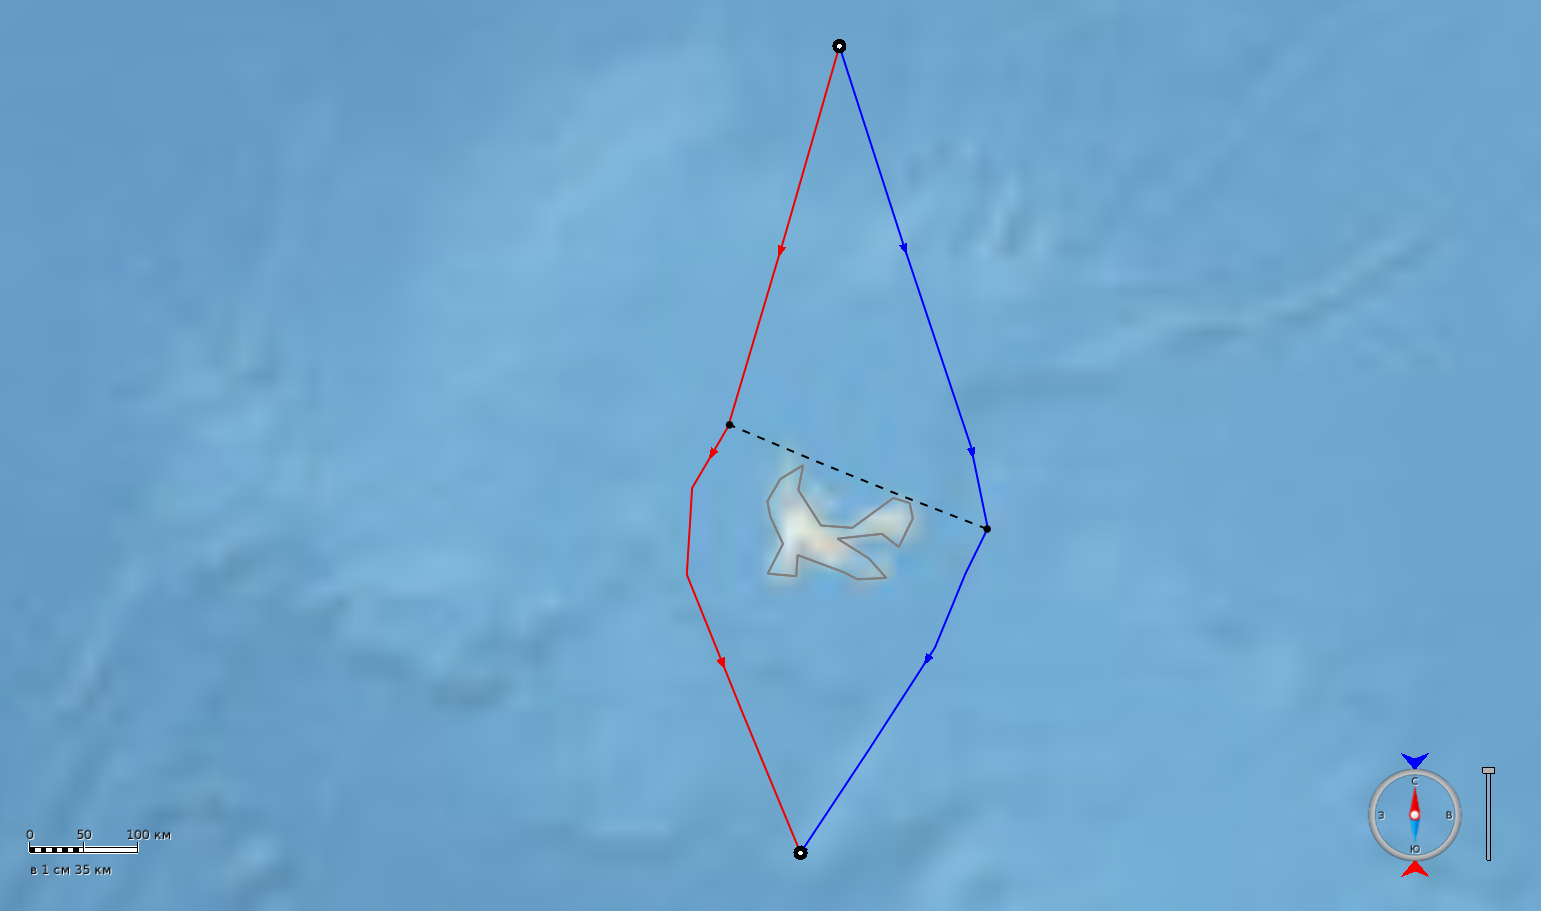
\includegraphics[width=.9\textwidth]{Solution/metrics/1-uncertain-2-dissimilar-closest}
            
            $\frac{\rho_1}{l_{min}} = \frac{307}{814} = 0.38$

            $\rho_2 = \frac{307}{251} = 1.22$
        \end{figure}
    }
    \only<6> {
        \begin{figure}
            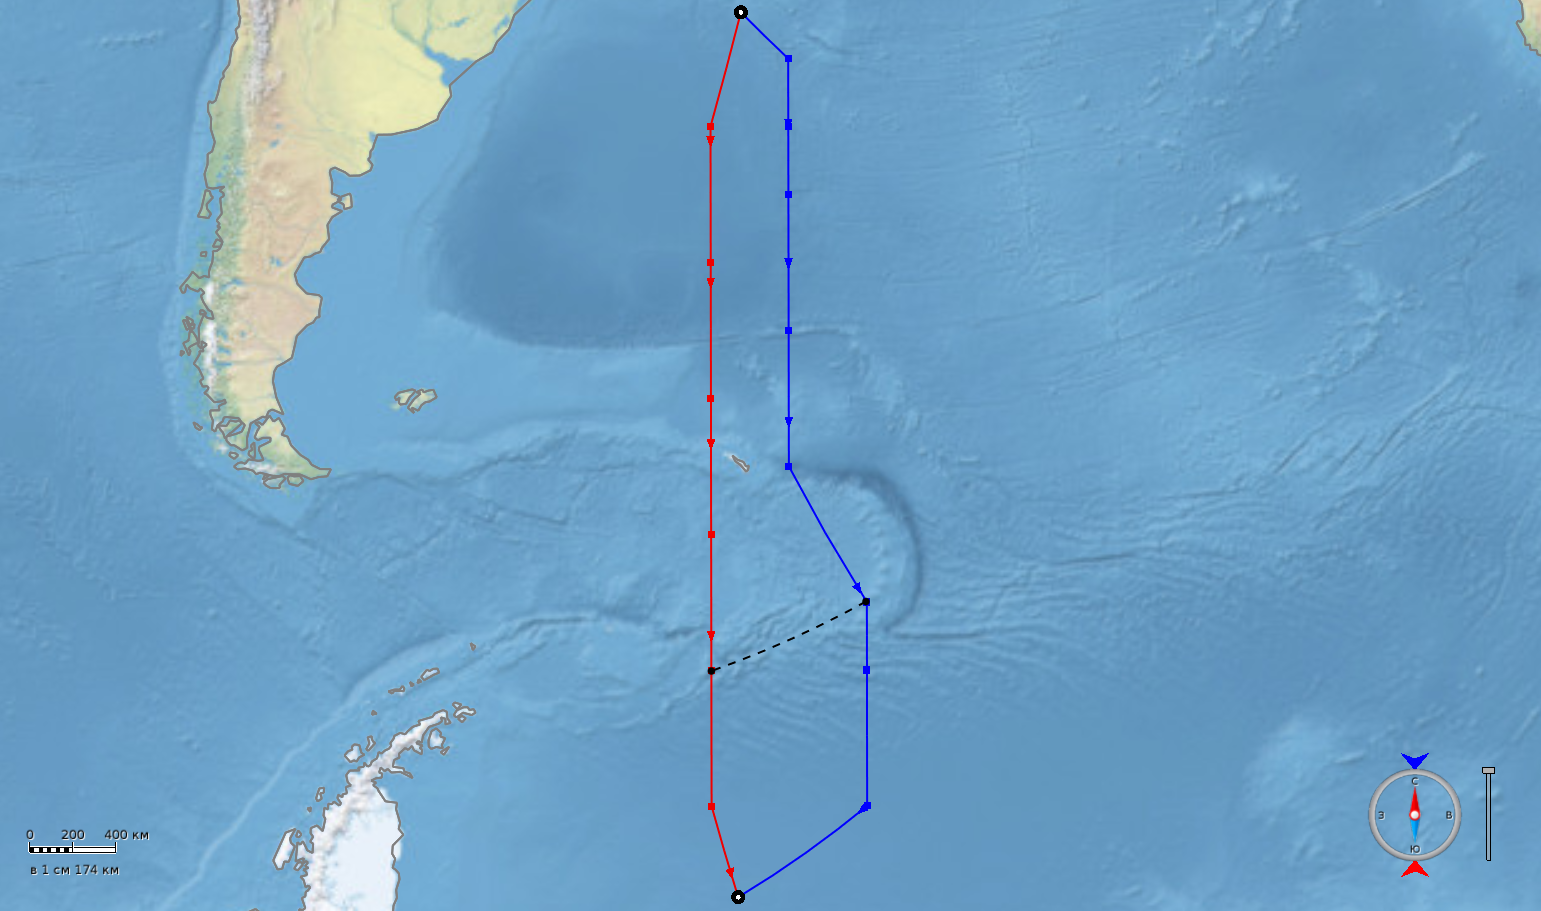
\includegraphics[width=.9\textwidth]{Solution/metrics/1-similar}
            
            $\frac{\rho_1}{l_{min}} = \frac{641}{4059} = 0.16$
        \end{figure}
    }
\end{frame}
\note {
Для оценки похожести будем использовать метрики на маршрутах.
Сказать, что такое $\rho_g$ и $\rho_r$.

Первая метрика берёт для каждой вершины первого пути кратчайшее расстояние до
ближайшей вершины второго пути, и её значение — максимум этих расстояний.
В зависимости от отношения её значения к длине кратчайшего из двух
путей маршруты считаются либо похожими, либо непохожими, либо
«возможно, похожими». В последнем случае используется вторая метрика.

Вторая метрика аналогична первой, но графовое расстояние до ближайшей
вершины в графе делится на реальное расстояние до ближайшей вершины в
мире. Большое значение этой метрики означает, что между путями есть
какое-то препятствие, поскольку кратчайший путь в графе существенно
больше реального расстояния до ближайшей вершины в мире. При этом не
рассматриваются  слишком близкие вершины, поскольку между ними может
быть незначительное препятствие.

Все скрытые константы являются параметрами алгоритма.
}

\section{Решение}

\subsection{Предобработка}

\begin{frame}{Предобработка данных}
    \begin{itemize}
        \item Карта → полигон
        \item Смещение полигона внутрь
        \item Граф по сетке на плоскости + граф локальной видимости
        \item Ограничение длины ребра
        \item Дополнительные рёбра
    \end{itemize}
\end{frame}
\note {
Чтобы искать пути, нужно построить граф.
\begin{itemize}
\item Контура в исходной карте упрощаются, чтобы в итоге было не очень
  много вершин в графе, и склеиваются, получается полигон, описывающий
  воду.
\item Полигон смещается внутрь, потому что корабли не плавают в
  12-мильной зоне и так будет лучше видно маршруты.
\item Затем строится граф по сетке на плоскости, то есть добавляются
  рёбра сетки, принадлежащие полигону. Также добавляются вершины
  полигона и рёбра из них во все видимые вершины в некотором радиусе.
\item При этом путь ищется на сфере, а проверка корректности рёбер
  осуществляется на плоскости. Кратчайшая траектория на сфере не
  является отрезком, поэтому не будем допускать слишком длинные рёбра,
  тогда расхождение будет пренебрежимо мало.
\item Также добавим рёбра, получившиеся в результате схлопывания
  отрезков при смещении полигона, и рёбра через 180-ый меридиан.
\end{itemize}
}

\subsection{Поиск}

\begin{frame}{Поиск одного маршрута}
    \only<1> {
        \begin{itemize}
            \item Добавление вершин в граф
            \item Алгоритм Дейкстры
            \item Сокращение маршрута
            \begin{itemize}
                \item Если подпуть A → B → C можно выгодно заменить на A → C, заменяем 
                \item Подразбиение маршрута
            \end{itemize}
            \item Сглаживание маршрута
        \end{itemize}
    }
    \only<2> {
        \begin{figure}
            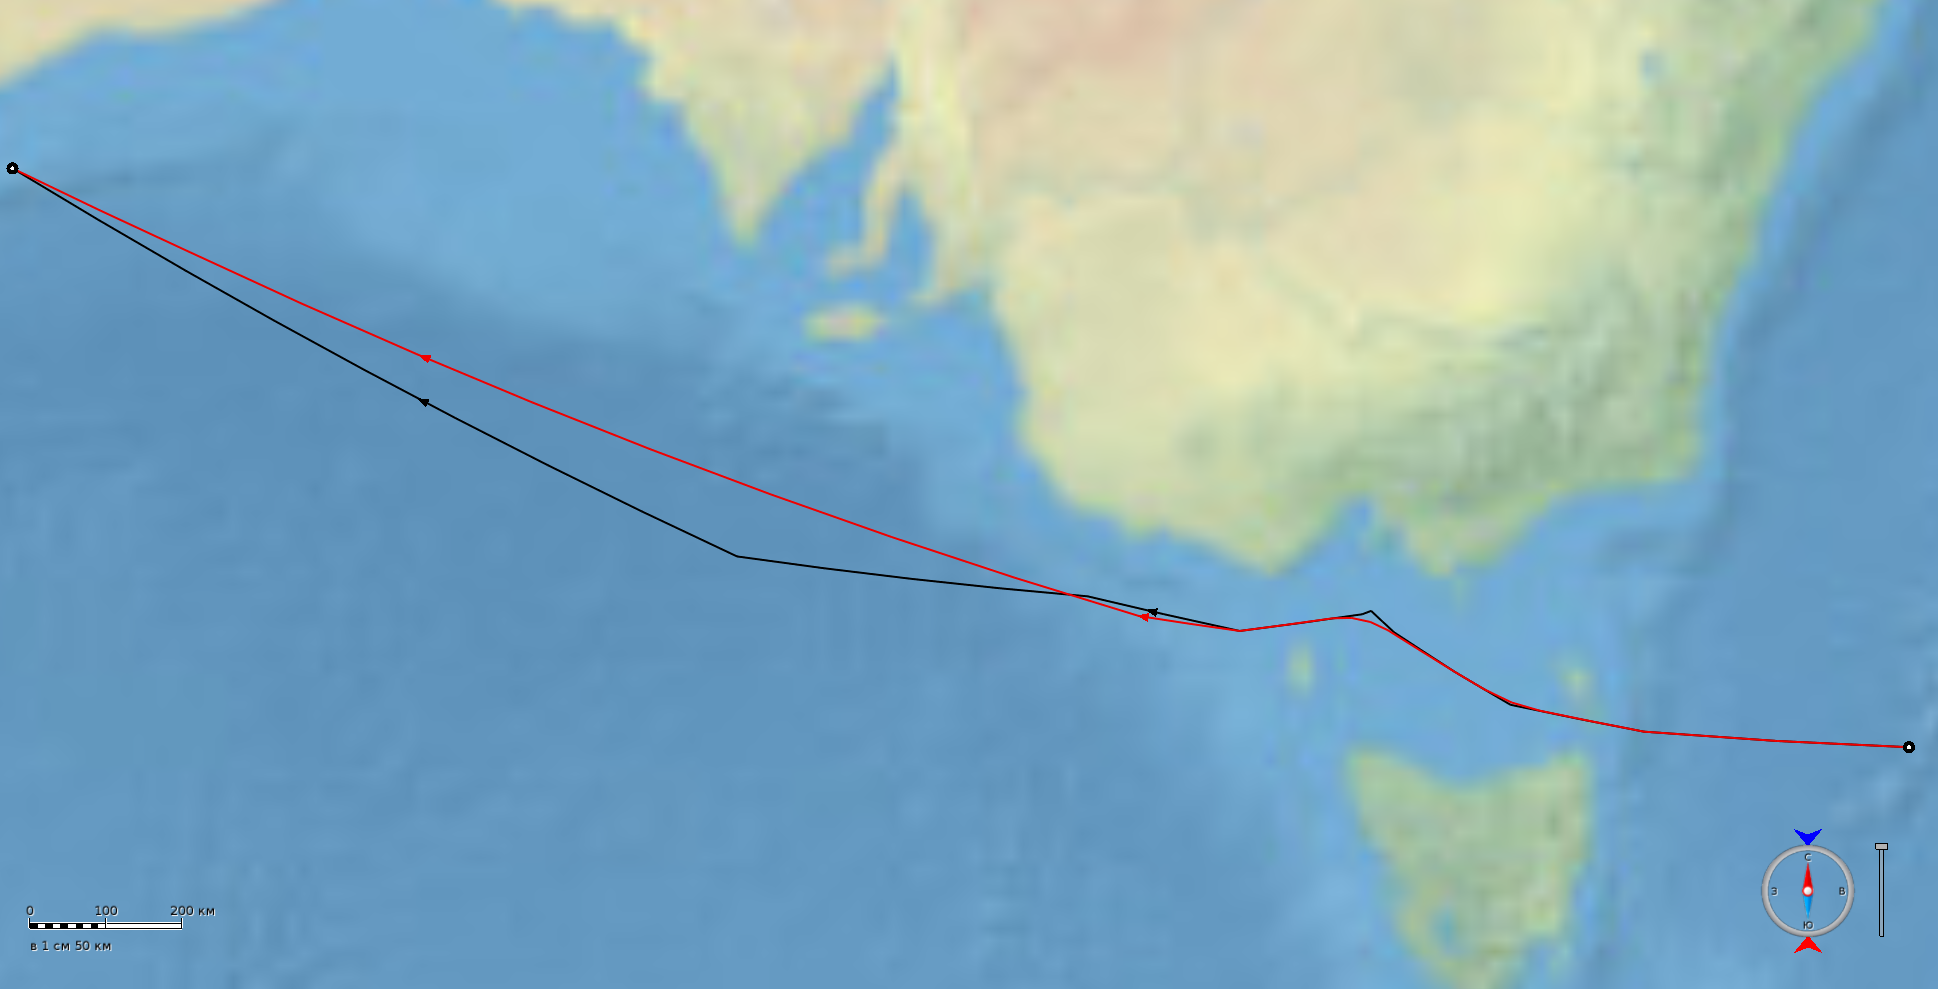
\includegraphics[width=\textwidth]{Solution/shortcut-and-smoothing}
            
            Сокращение и сглаживание
        \end{figure}
    }
\end{frame}
\note {
Перейдём к описанию поиска. Начнём с описания поиска одного
маршрута, поскольку он лежит в основе поиска семейств маршрутов.

\begin{itemize}
\item
Сначала происходит добавление вершин в граф и рёбер до ближайших
вершин, находимых по сетке.
\item
Сам поиск пути осуществляется с помощью алгоритма Дейкстры.
\item
Поскольку граф не является графом видимости, то кратчайший путь в нём
не обязан быть действительно кратчайшим путём между двумя точками.
Обычно его можно сократить. Дальше по тексту.
\item
В связи со структурой графа возможно появление слишком острых углов в
маршруте, которые выглядят неестественно, поэтому выполняется их сглаживание.
\end{itemize}

Про рисунок всё понятно: слева сократилось, справа сгладилось.
}

\subsection{Поиск нескольких маршрутов}

\begin{frame}{Поиск нескольких маршрутов}
    \begin{algorithmic}
        \Function{find\_paths}{}
            \State p, len $\gets$ find\_path()
            \State paths $\gets$ \{p\}
            \State min\_len $\gets$ len
            \While{paths.size() < max\_paths\_count}
                \State update\_weigths(p, len)
                \State p, len $\gets$ find\_path()
                \If{$len > C_0 \cdot min\_len$}
                    \State \Return paths
                \EndIf
                \For{q in paths}:
                    \If{similar(p, q)}
                        \State \Return paths
                    \EndIf
                \EndFor

                \State paths.insert(p)
           \EndWhile
        \EndFunction
     \end{algorithmic}
\end{frame}
\note {
Поиск нескольких маршрутов проиллюстрируем псевдокодом.

Сначала находится кратчайший путь описанным только что способом, он
добавляется в результат, запоминается длина. Затем, пока не найдено
слишком много маршрутов, делаем следующее: обновляем веса в графе (об
этом будем сказано на следующем слайде), находим очередной маршрут.
Если его длина слишком большая, то заканчиваем. Также заканчиваем,
если среди среди имеющихся маршрутов имеется похожий на только что
найденный в смысле описанных ранее метрик. Наконец, если маршрут
хороший, то он добавляется в результат.
}

\begin{frame}{Обновление весов}
     \begin{algorithmic}
        \Function{update\_weights}{p, len}
            \State g' $\gets$ graph\_with\_fake(p)
            \State limit $\gets \frac{len}{C_1}$
            \State d $\gets$ shortest\_in\_radius(g', fake, limit)
            \ForAll{v in vertices}
            \State potential = $1 + (max\_potential - 1) \cdot \frac{limit - d[v]}{limit}$
            \State pot[v] = max(pot[v], potential)
            \EndFor
            \ForAll{e in edges}
            \State e.weight = $e.initial\_weight \cdot
            \sqrt{pot[e.from] \cdot  pot[e.to]}$
            \EndFor
        \EndFunction
     \end{algorithmic}
\end{frame}
\note {
Теперь об обновлении весов. Для каждой вершины храним потенциал. Чем
он больше, тем сильнее будет увеличен вес инцидентных рёбер. При
обновлении сначала построим новый граф с фиктивной вершиной, из
которой проведены рёбра нулевого веса во все вершины пути. Затем с
помощью алгоритма Дейкстры найдём кратчайшие расстояния из фиктивной
вершины до всех остальных в этом графе в радиусе равном длине пути,
поделённой на константу. Для всех вершин посчитаем новый потенциал как
число от одного до максимального потенциала. Чем больше расстояние до
пути, тем меньше потенциал. обновим потенциалы всех вершин, взяв
максимум. Обновим веса рёбер, взяв начальный вес, умноженный на
среднее геометрическое потенциалов смежных вершин.
}

\begin{frame}{Вычисление метрик}
    \begin{itemize}
        \item Фиктивная вершина
        \item Обход Дейкстры, пока не посещены вершины второго пути 
        \item Заканчиваем, если достигли необходимого значения
        \item Поиск ближайшей вершины (вторая метрика) — перебором
        \item На практике затраты как на первую, так и на вторую
          метрику небольшие
    \end{itemize}
\end{frame}
\note {
Тут вроде понятно
}

\section{Результаты}

\begin{frame}{Результаты}
    \only<1> {
        \begin{itemize}
            \item На основе предложенного алгоритма разработан программный модуль,
              решающий задачу построения требуемых семейств маршрутов
            \item Время поиска не превышает одну секунду
            \item Используется в 3D-клиенте ЗАО «Кронштадт Технологии»
            \item Получено заключение экспертов ЗАО «ОСК-Транзас», подтверждающее,
              что разработанный программный модуль удовлетворяет предъявленным
              требованиям
        \end{itemize}
    }
    \only<2> {
        \begin{figure}
            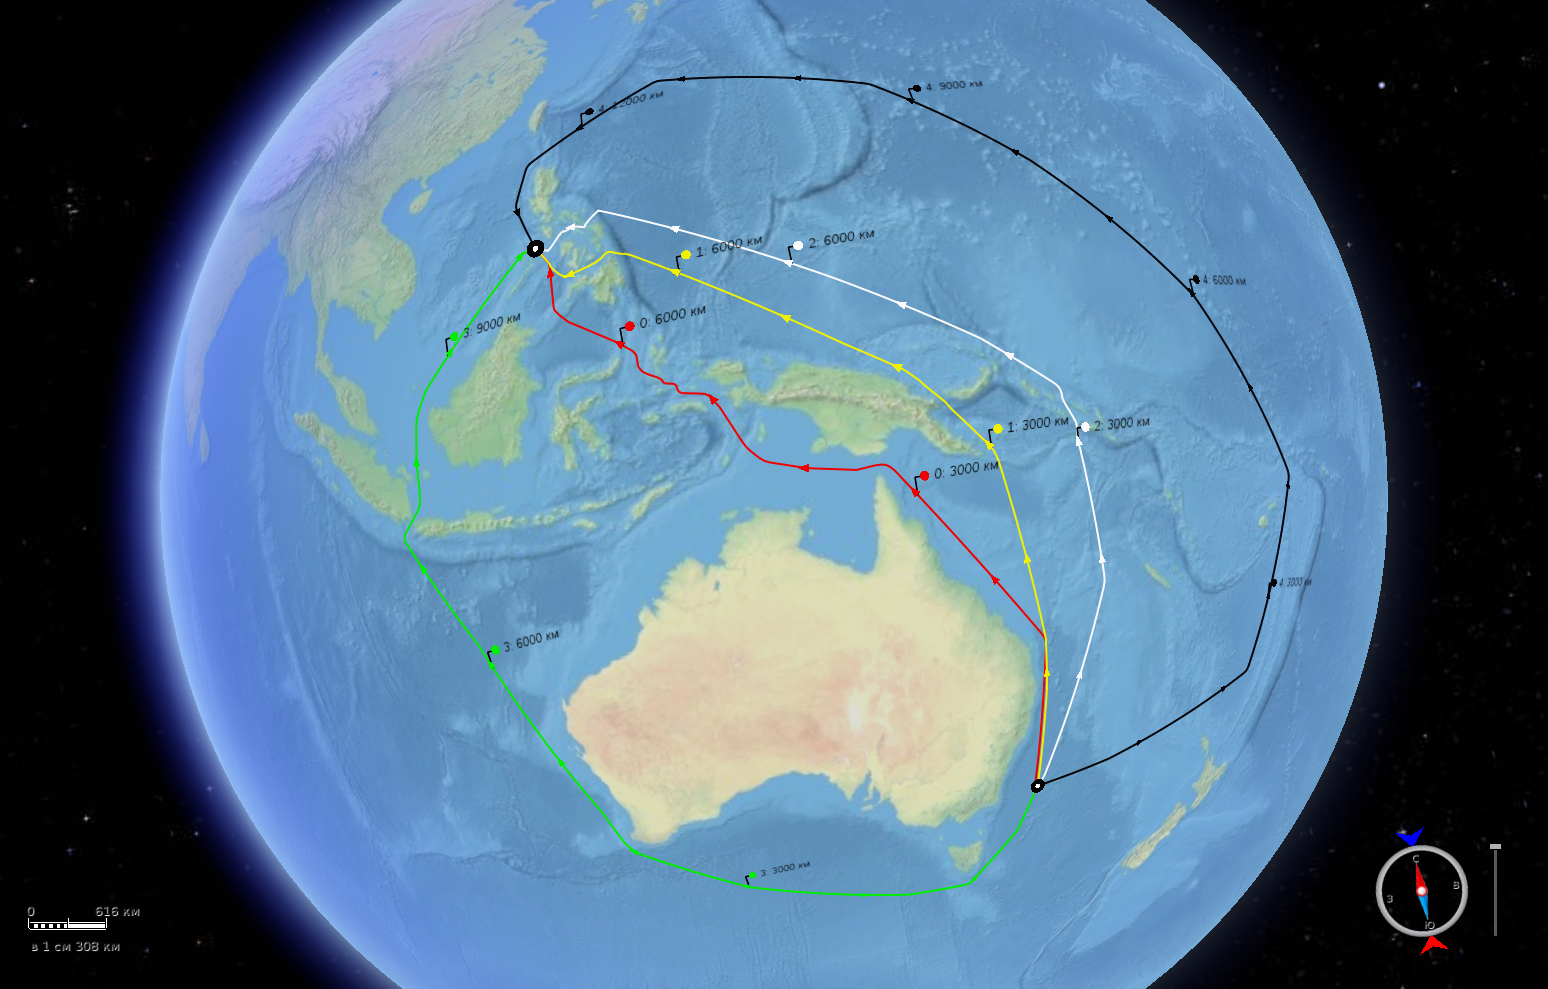
\includegraphics[width=\textwidth]{Results/1}
        \end{figure}
    }

    \only<3> {
        \begin{figure}
            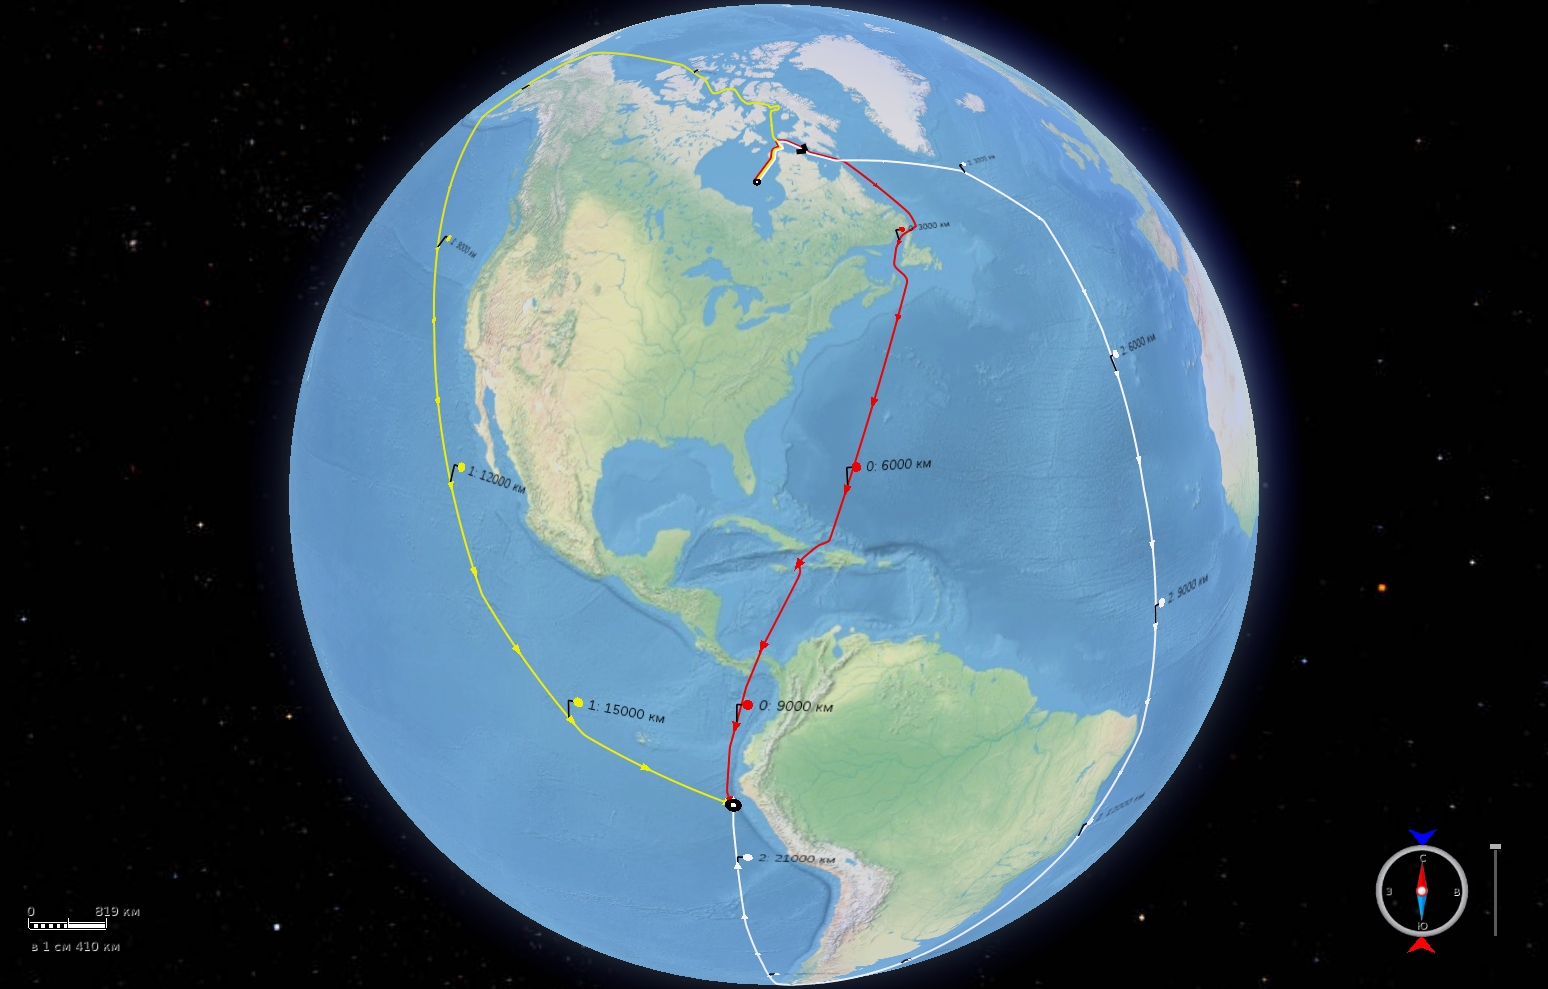
\includegraphics[width=\textwidth]{Results/2}
        \end{figure}
    }

    \only<4> {
        \begin{figure}
            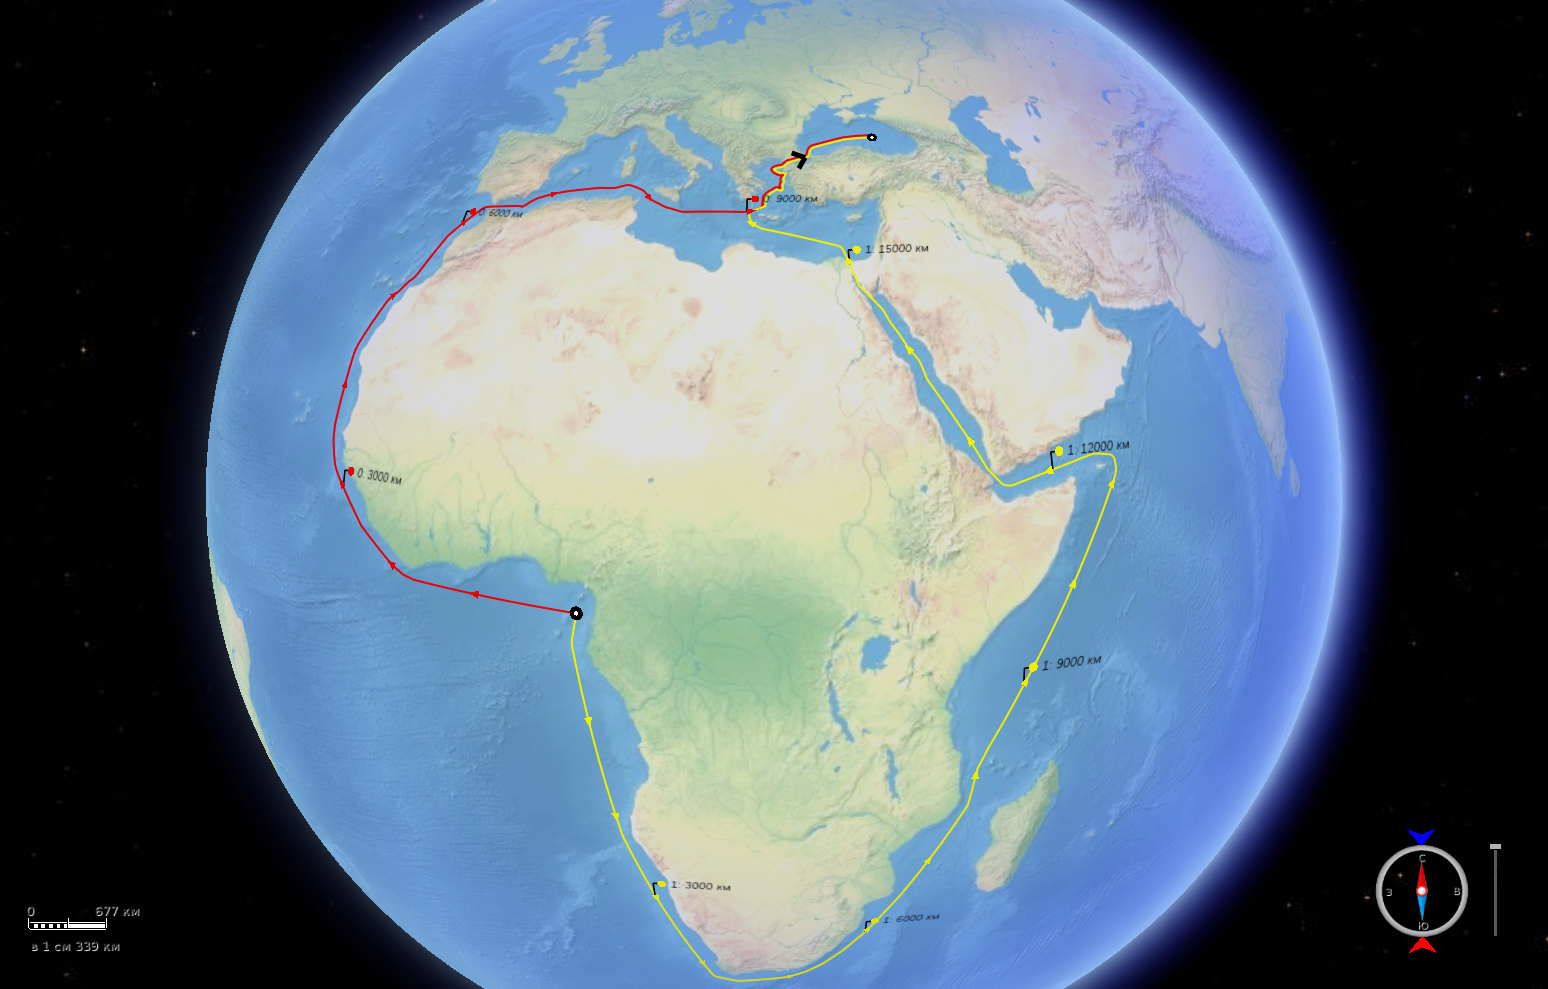
\includegraphics[width=\textwidth]{Results/3}
        \end{figure}
    }

\end{frame}
\note {
Типа вот вам результаты, всё круто, я хорош.
}

\begin{frame}{Спасибо за внимание!}
    \begin{center}
        \Huge
        {\color{blue} Вопросы?}
    \end{center}
\end{frame}
\note{До свидания!}

\appendix

\begin{frame}[noframenumbering]{Обновление весов}
    \only<1> {
        \begin{figure}
            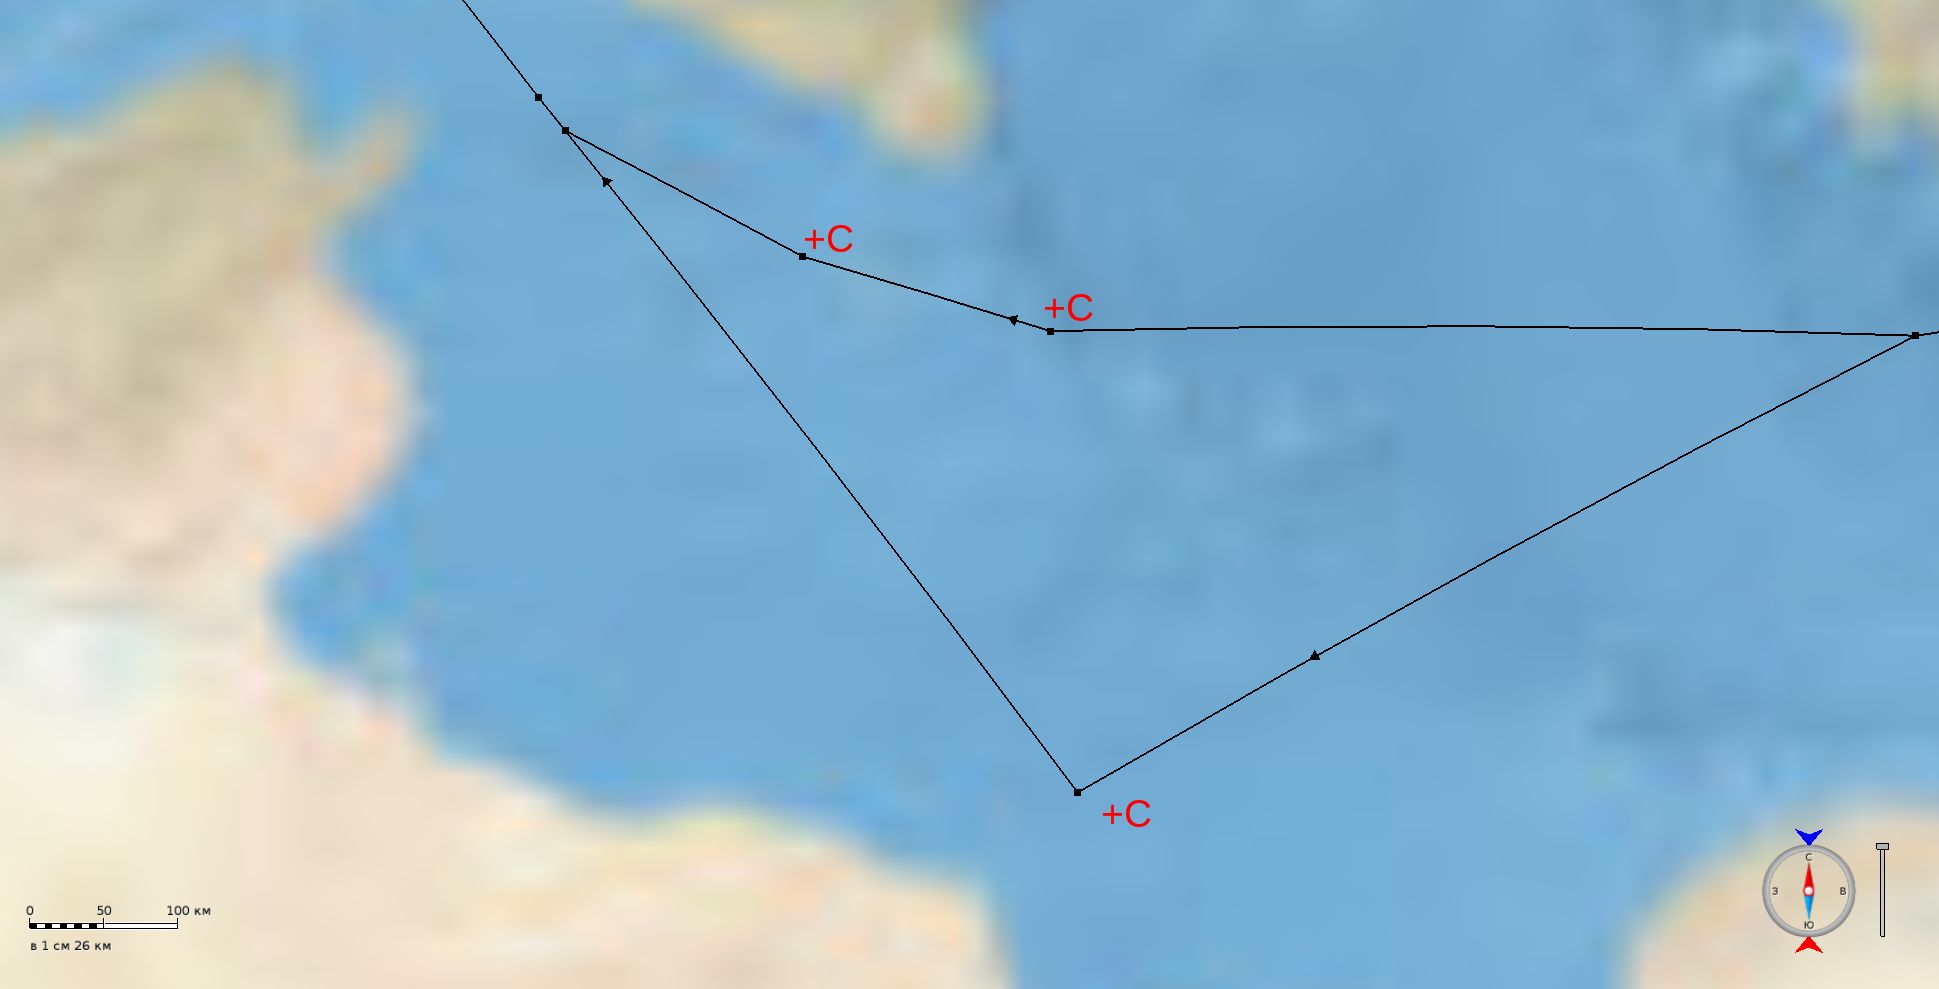
\includegraphics[width=\textwidth]{Solution/potentials-multipliers}

            Потенциалы должны быть множителями, а не слагаемыми
        \end{figure}
    }
 
    \only<2> {
        \begin{columns}
            \column{.5\textwidth}
            \begin{figure}
                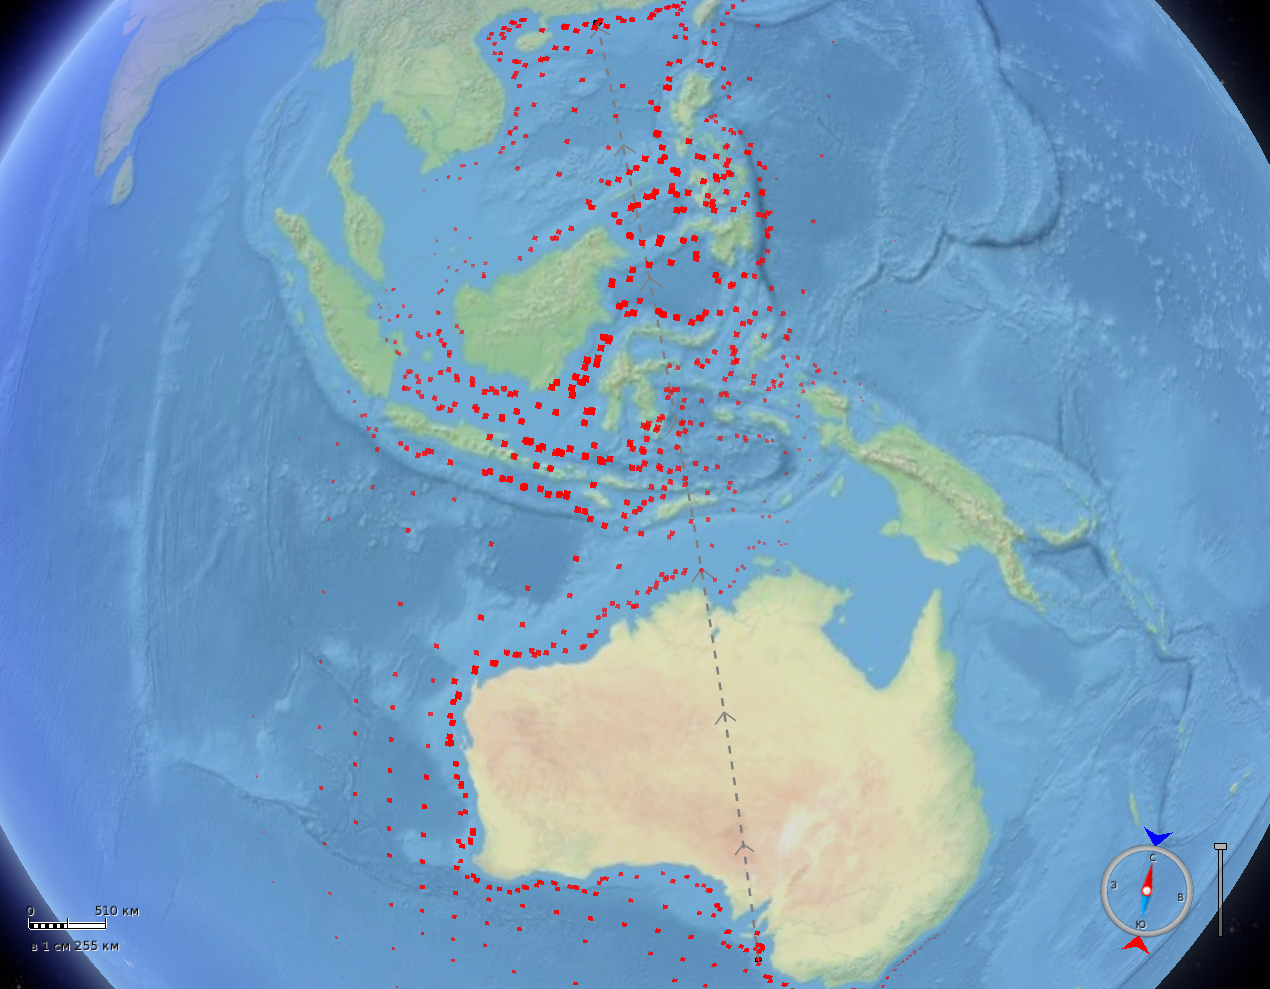
\includegraphics[clip=true, trim = 280pt 0 20pt 0, width=\textwidth]{Solution/potentials-update/accum1}
            \end{figure}

            \column{.5\textwidth}
            \begin{figure}
                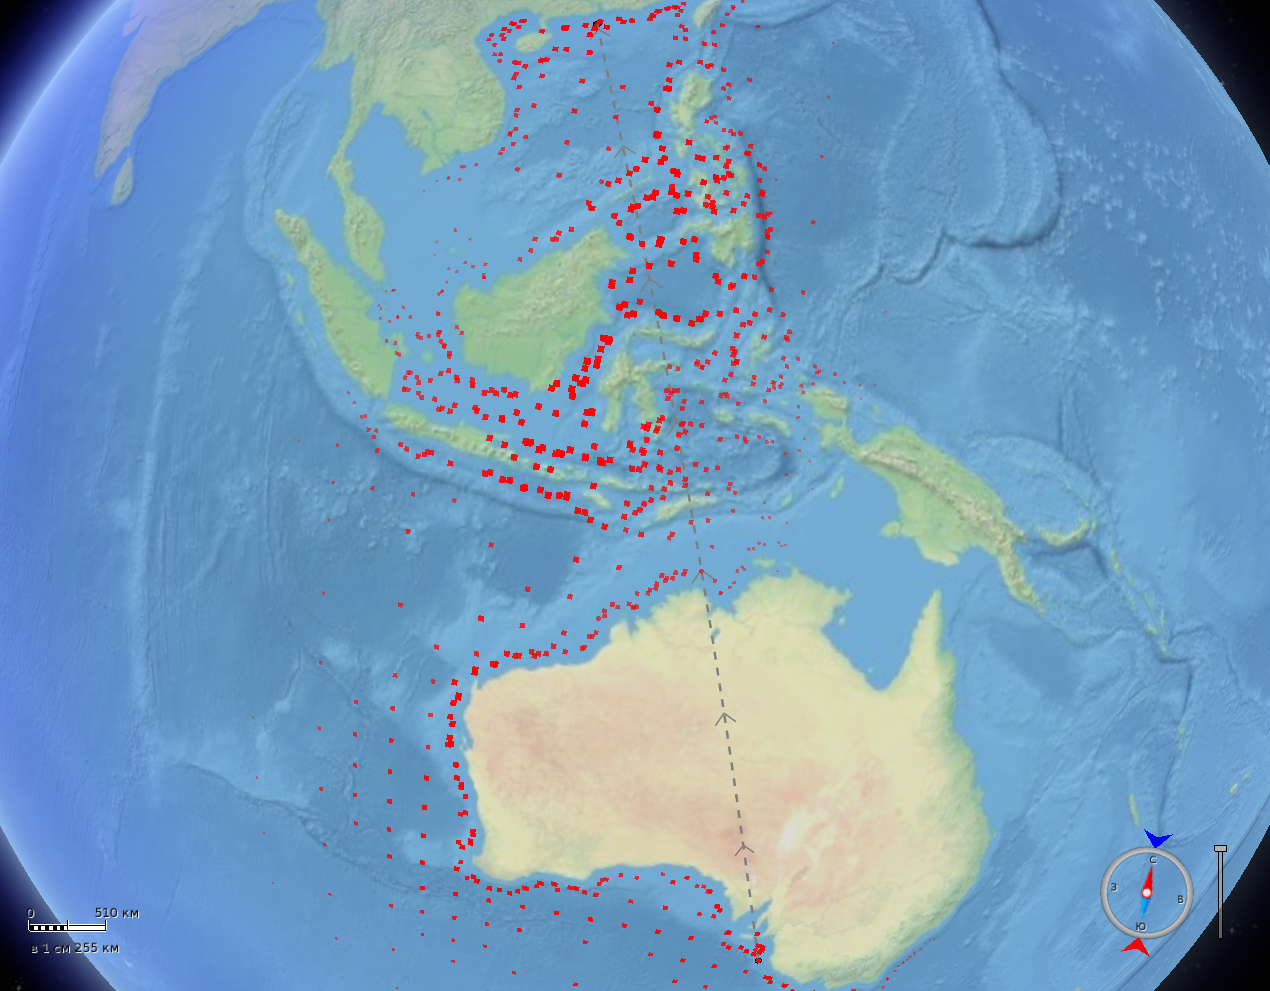
\includegraphics[clip=true, trim = 280pt 0 20pt 0, width=\textwidth]{Solution/potentials-update/max1}
            \end{figure}
        \end{columns}

        \begin{center}
            При обновлении потенциалов следует брать максимум.
        \end{center}
    }
   
    \only<3> {
        \begin{columns}
            \column{.5\textwidth}
            \begin{figure}
                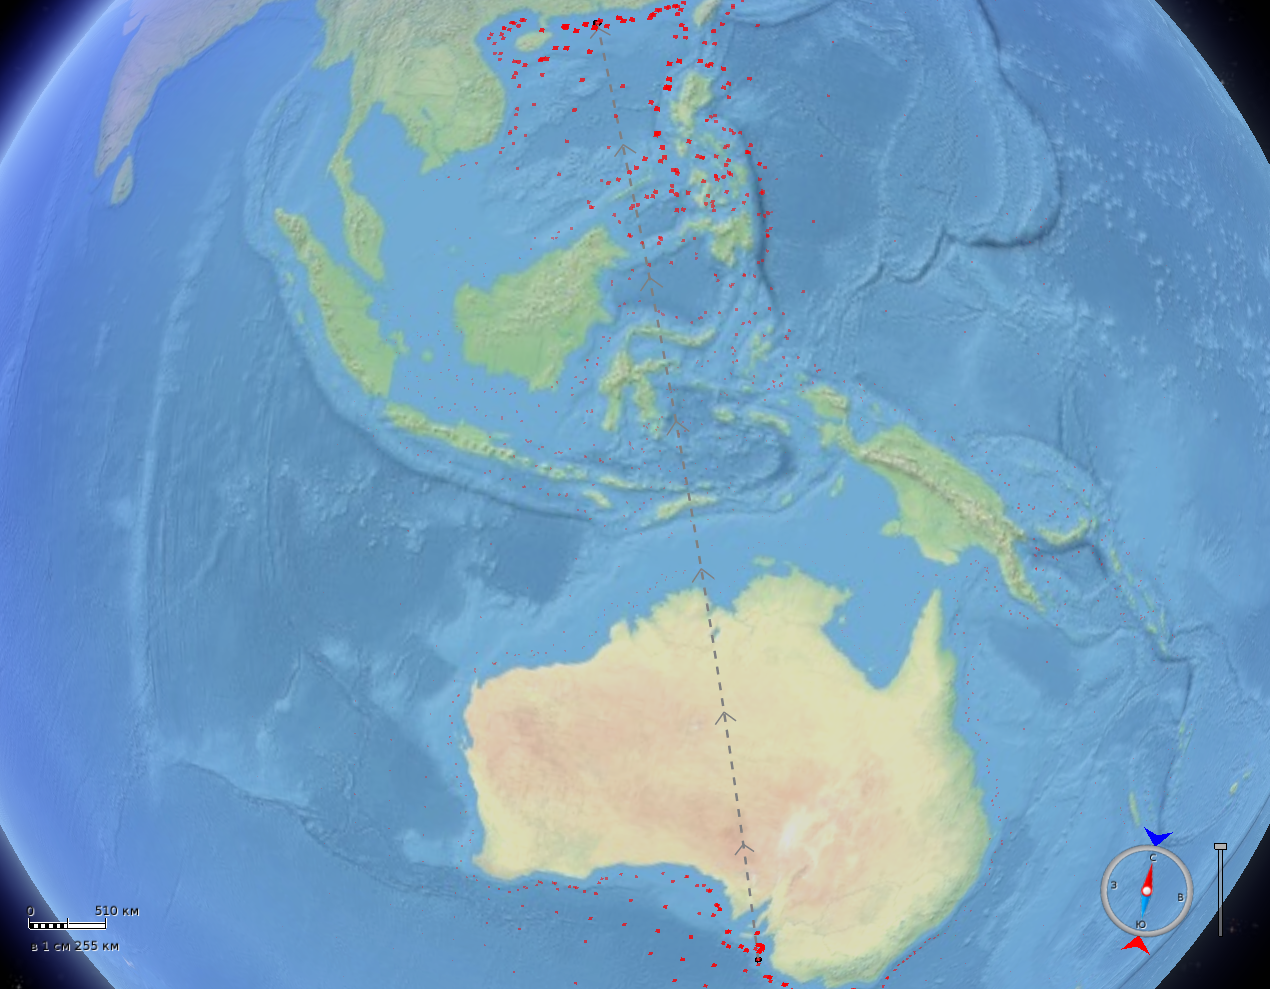
\includegraphics[clip=true, trim = 280pt 0 20pt 0, width=\textwidth]{Solution/potentials-update/accum2}
            \end{figure}

            \column{.5\textwidth}
            \begin{figure}
                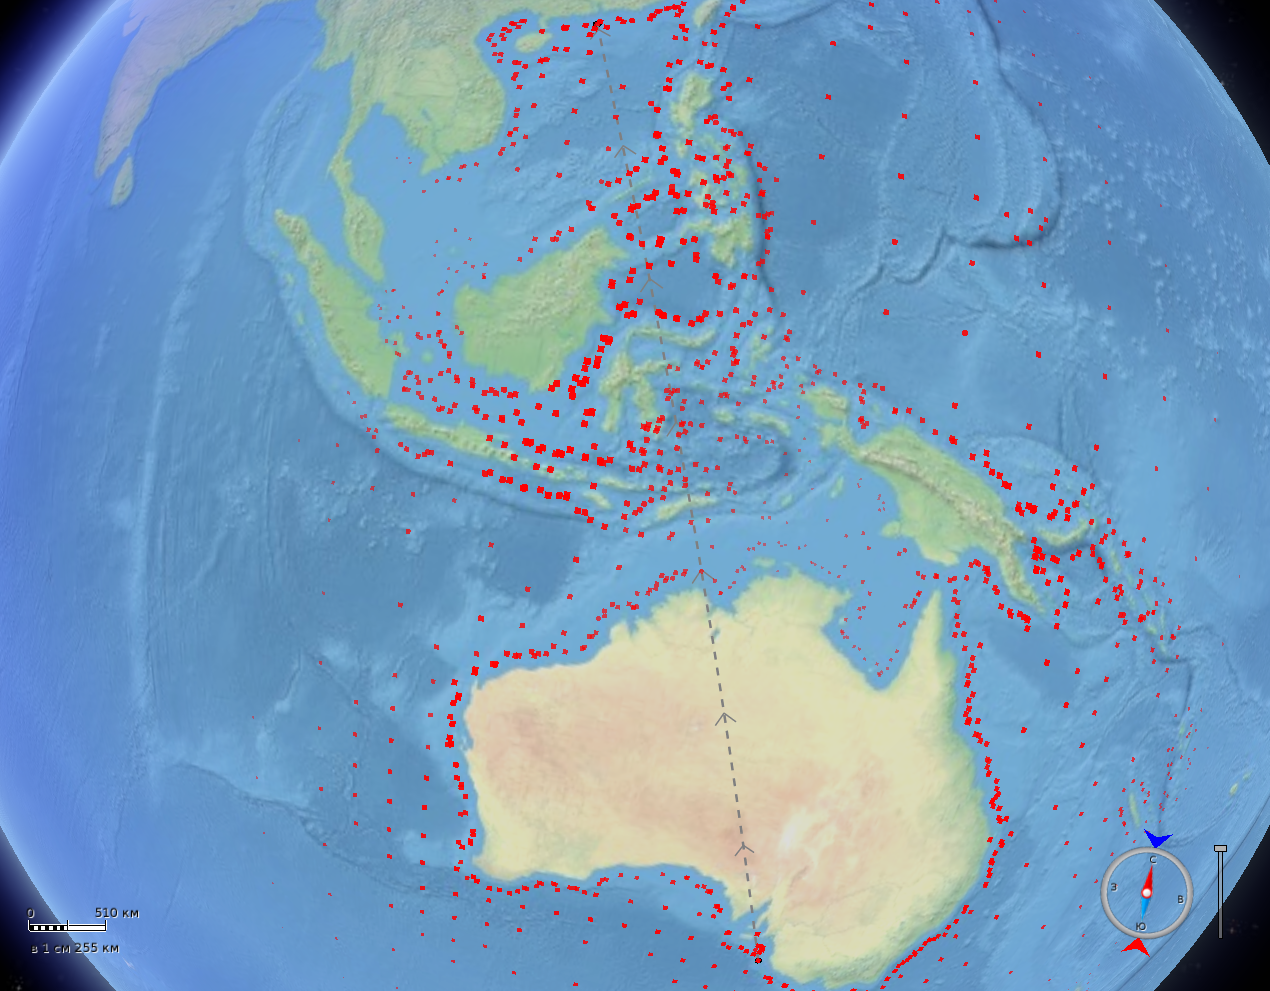
\includegraphics[clip=true, trim = 280pt 0 20pt 0, width=\textwidth]{Solution/potentials-update/max2}
            \end{figure}
        \end{columns}

        \begin{center}
            При обновлении потенциалов следует брать максимум.
        \end{center}
    }
   
    \only<4> {
        \begin{columns}
            \column{.5\textwidth}
            \begin{figure}
                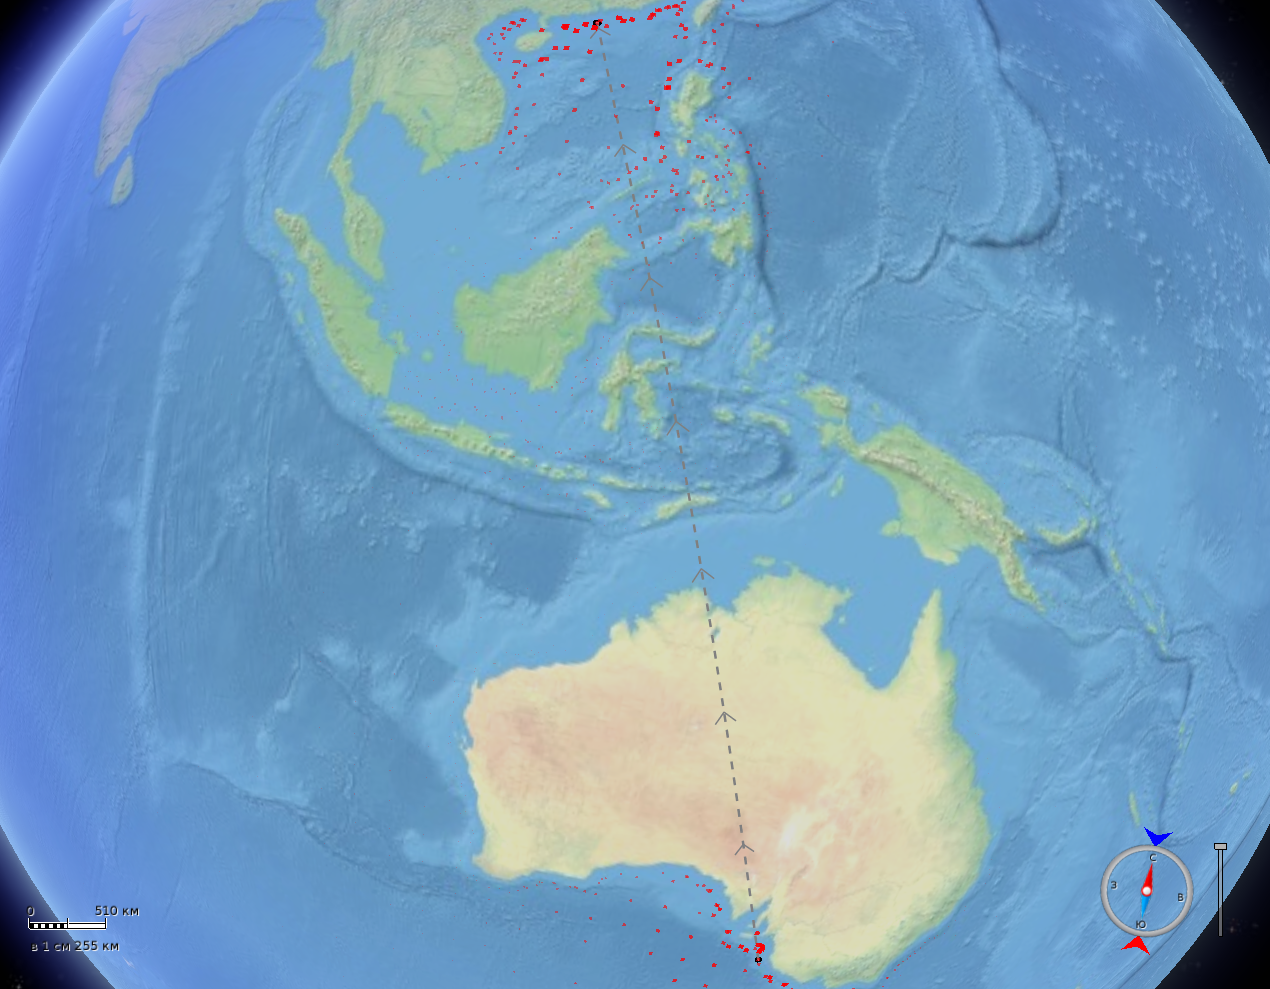
\includegraphics[clip=true, trim = 280pt 0 20pt 0, width=\textwidth]{Solution/potentials-update/accum3}
            \end{figure}

            \column{.5\textwidth}
            \begin{figure}
                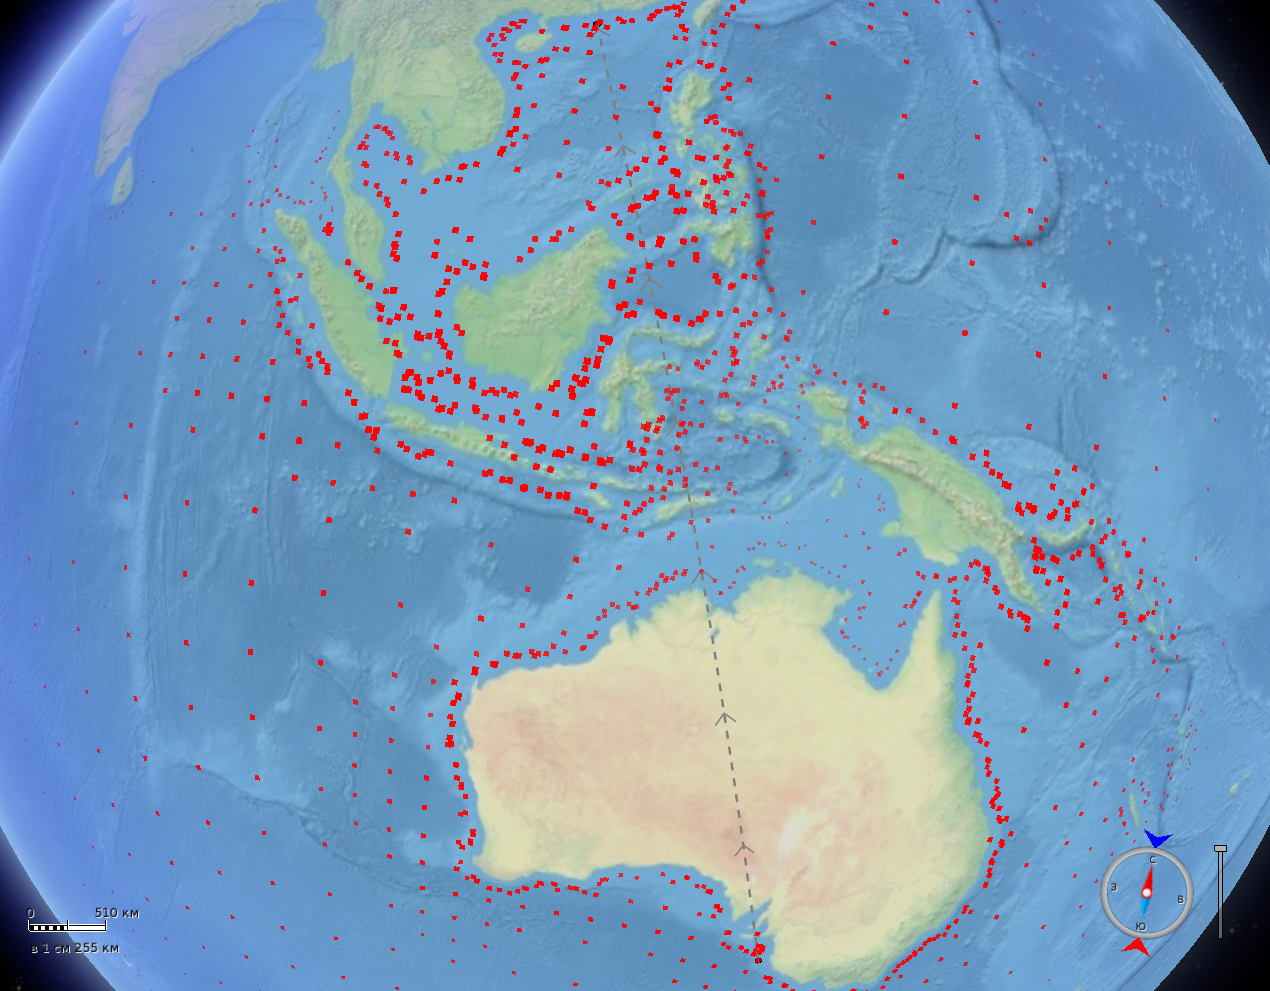
\includegraphics[clip=true, trim = 280pt 0 20pt 0, width=\textwidth]{Solution/potentials-update/max3}
            \end{figure}
        \end{columns}
        
        \begin{center}
            При обновлении потенциалов следует брать максимум.
        \end{center}
    }
   
    \only<5> {
        \begin{columns}
            \column{.5\textwidth}
            \begin{figure}
                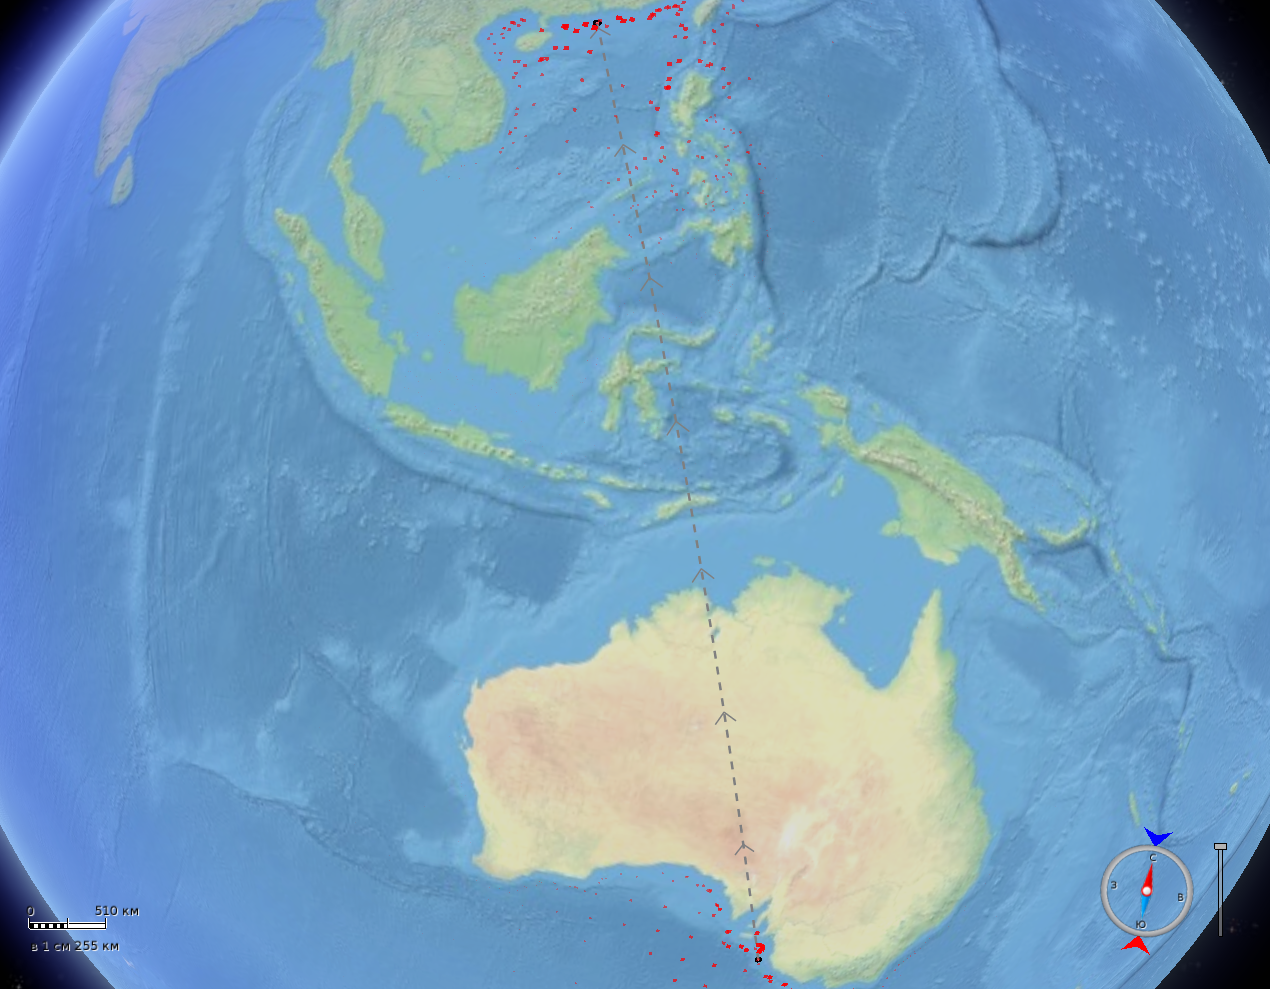
\includegraphics[clip=true, trim = 280pt 0 20pt 0, width=\textwidth]{Solution/potentials-update/accum4}
            \end{figure}

            \column{.5\textwidth}
            \begin{figure}
                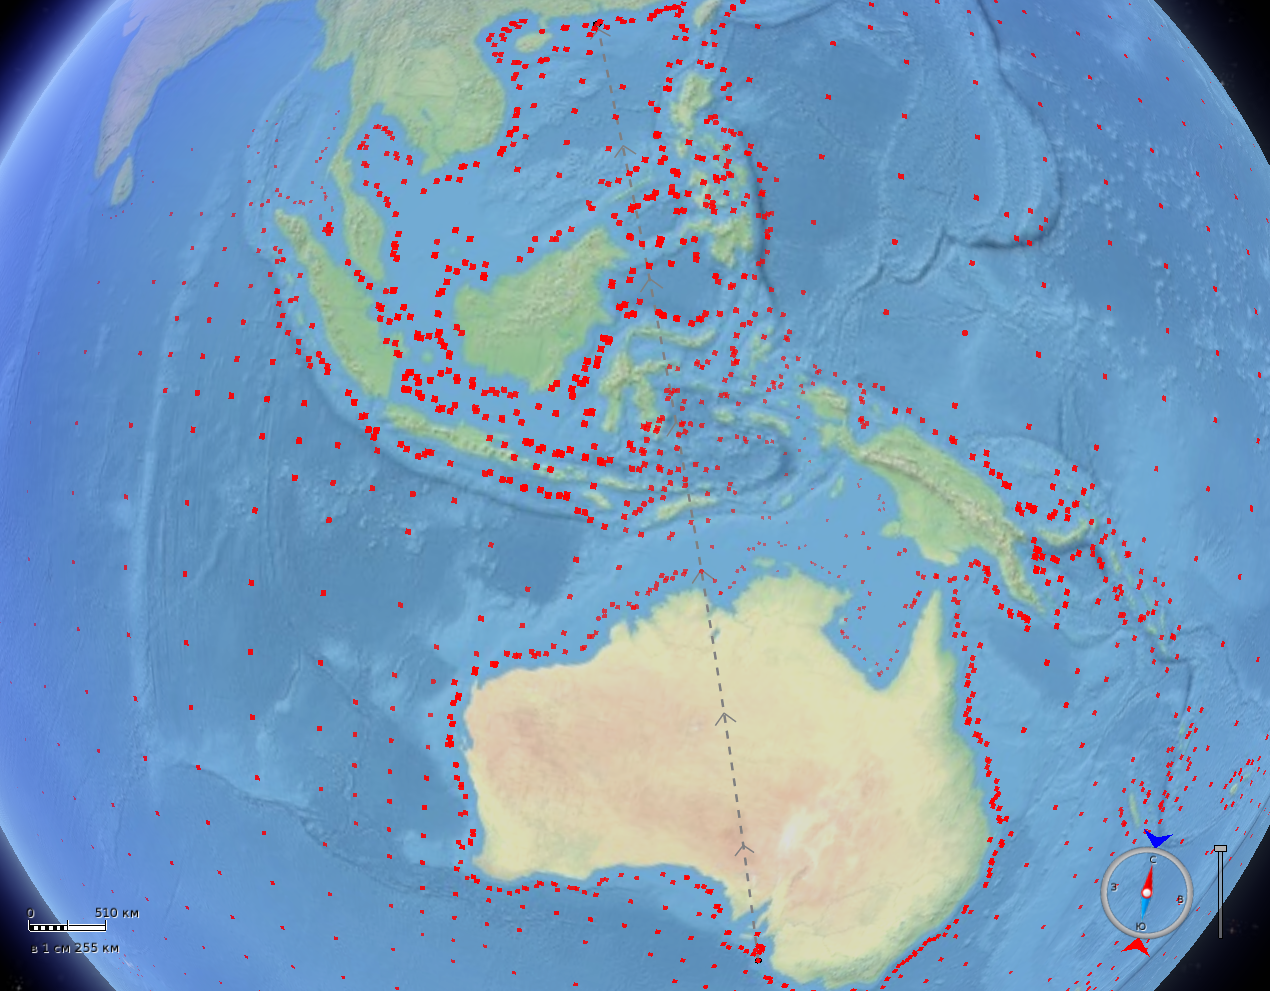
\includegraphics[clip=true, trim = 280pt 0 20pt 0, width=\textwidth]{Solution/potentials-update/max4}
            \end{figure}
        \end{columns}
        
        \begin{center}
            При обновлении потенциалов следует брать максимум.
        \end{center}
    }
   
    \only<6> {
        \begin{columns}
            \column{.5\textwidth}
            \begin{figure}
                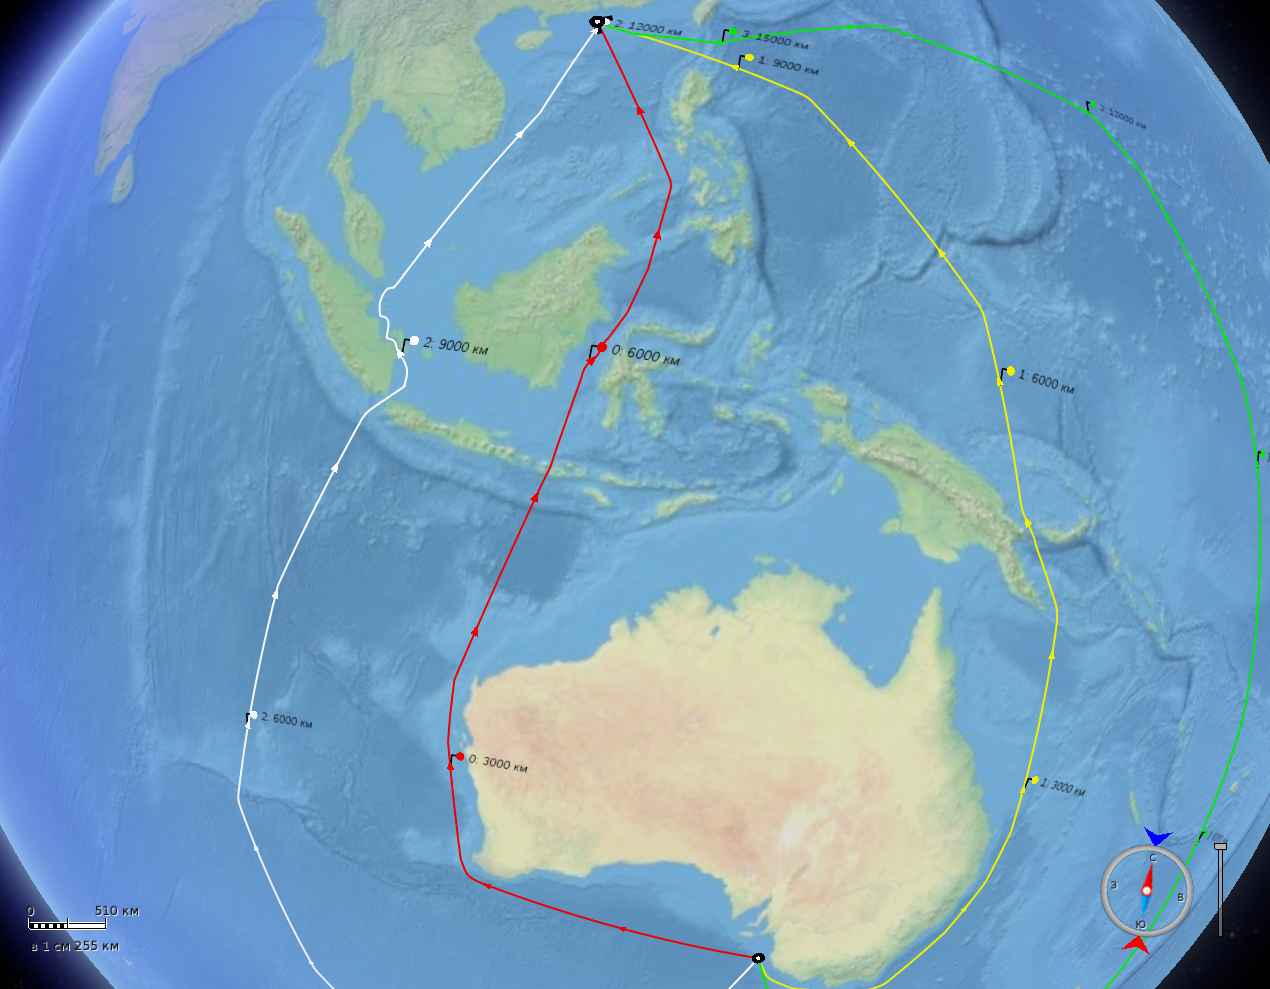
\includegraphics[clip=true, trim = 280pt 0 20pt 0, width=\textwidth]{Solution/potentials-update/accum_result}
            \end{figure}

            \column{.5\textwidth}
            \begin{figure}
                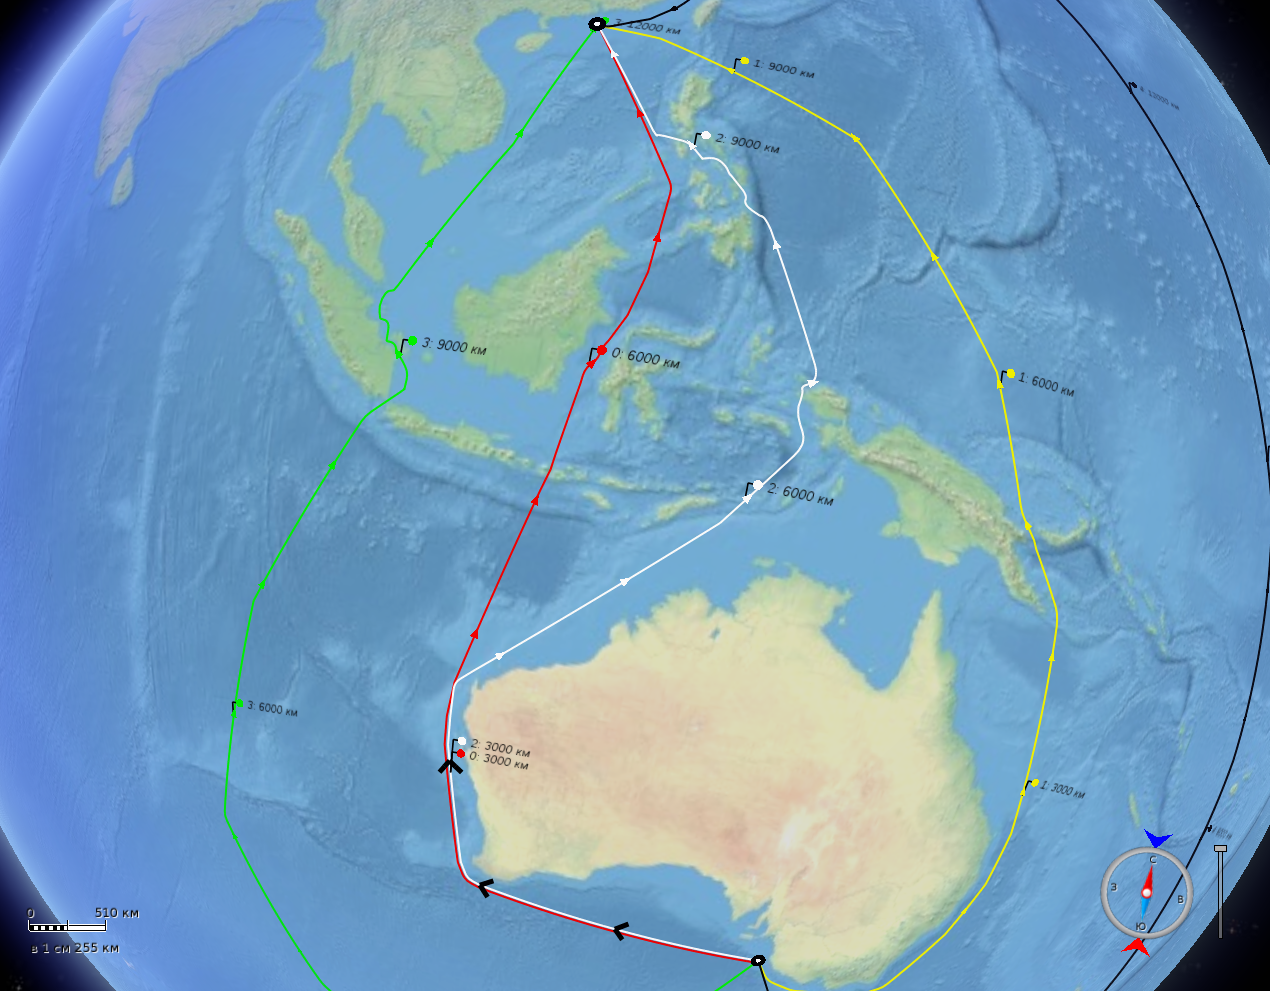
\includegraphics[clip=true, trim = 280pt 0 20pt 0, width=\textwidth]{Solution/potentials-update/max_result}
            \end{figure}
        \end{columns}
        
        \begin{center}
            При обновлении потенциалов следует брать максимум.
        \end{center}
    }
   
    \only<7> {
        \begin{figure}
          \begin{columns}
            \column{.5\textwidth}
            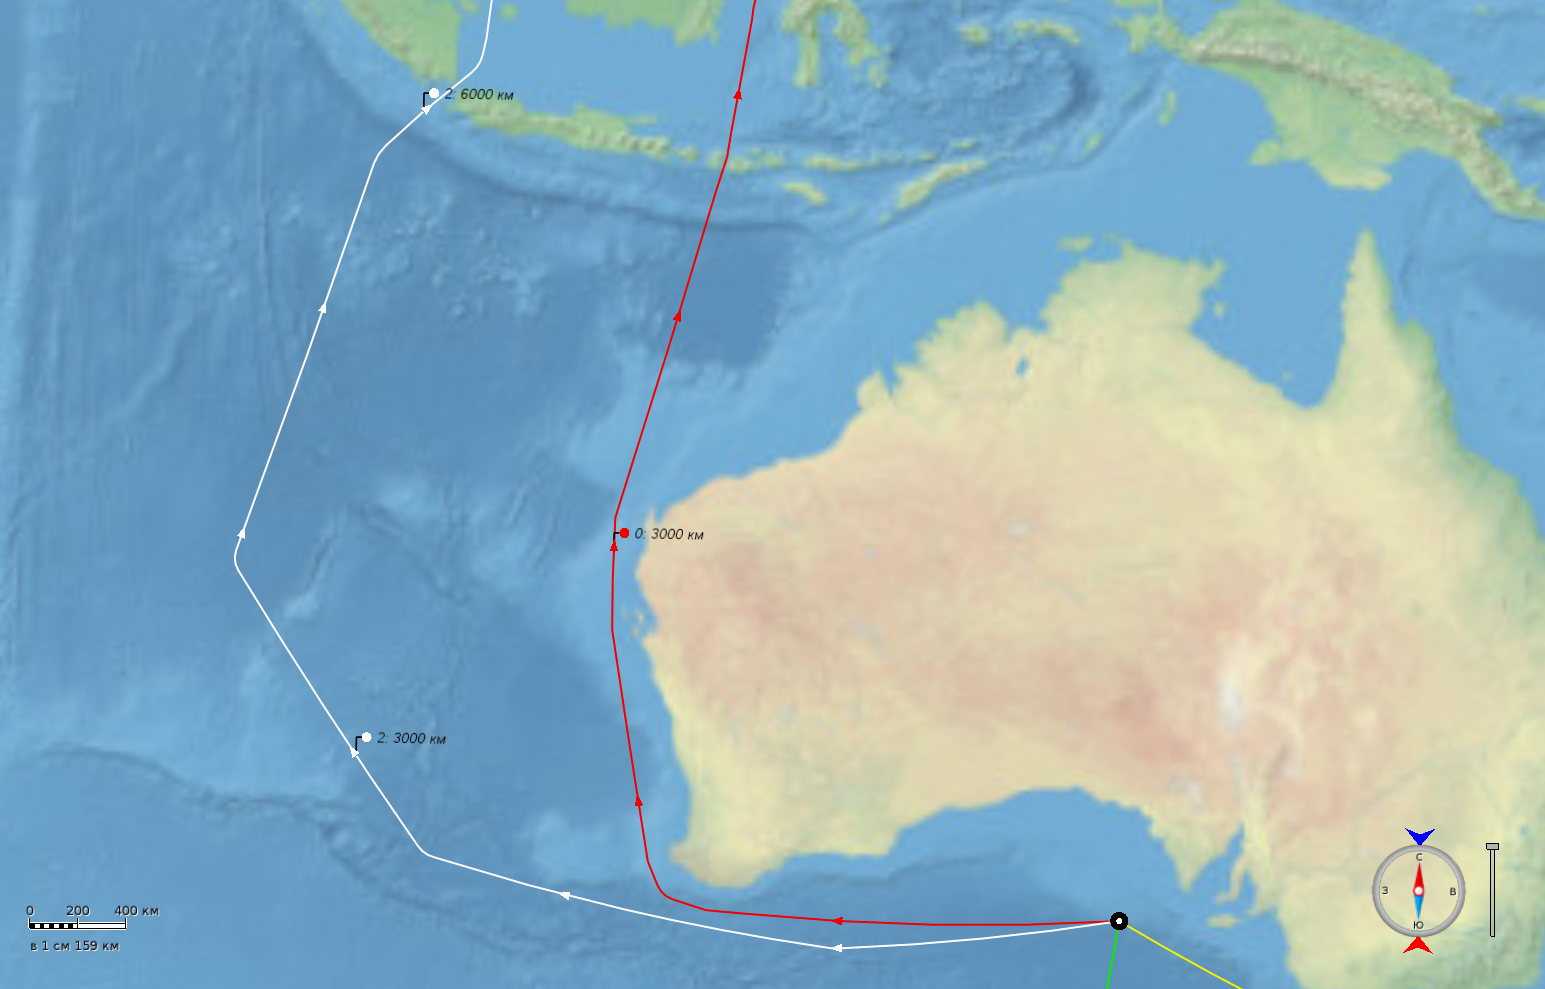
\includegraphics[clip=true, trim = 300pt 20pt 330pt 350pt, width=\textwidth]{Solution/weights-on-path-bad}

            \column{.5\textwidth}
            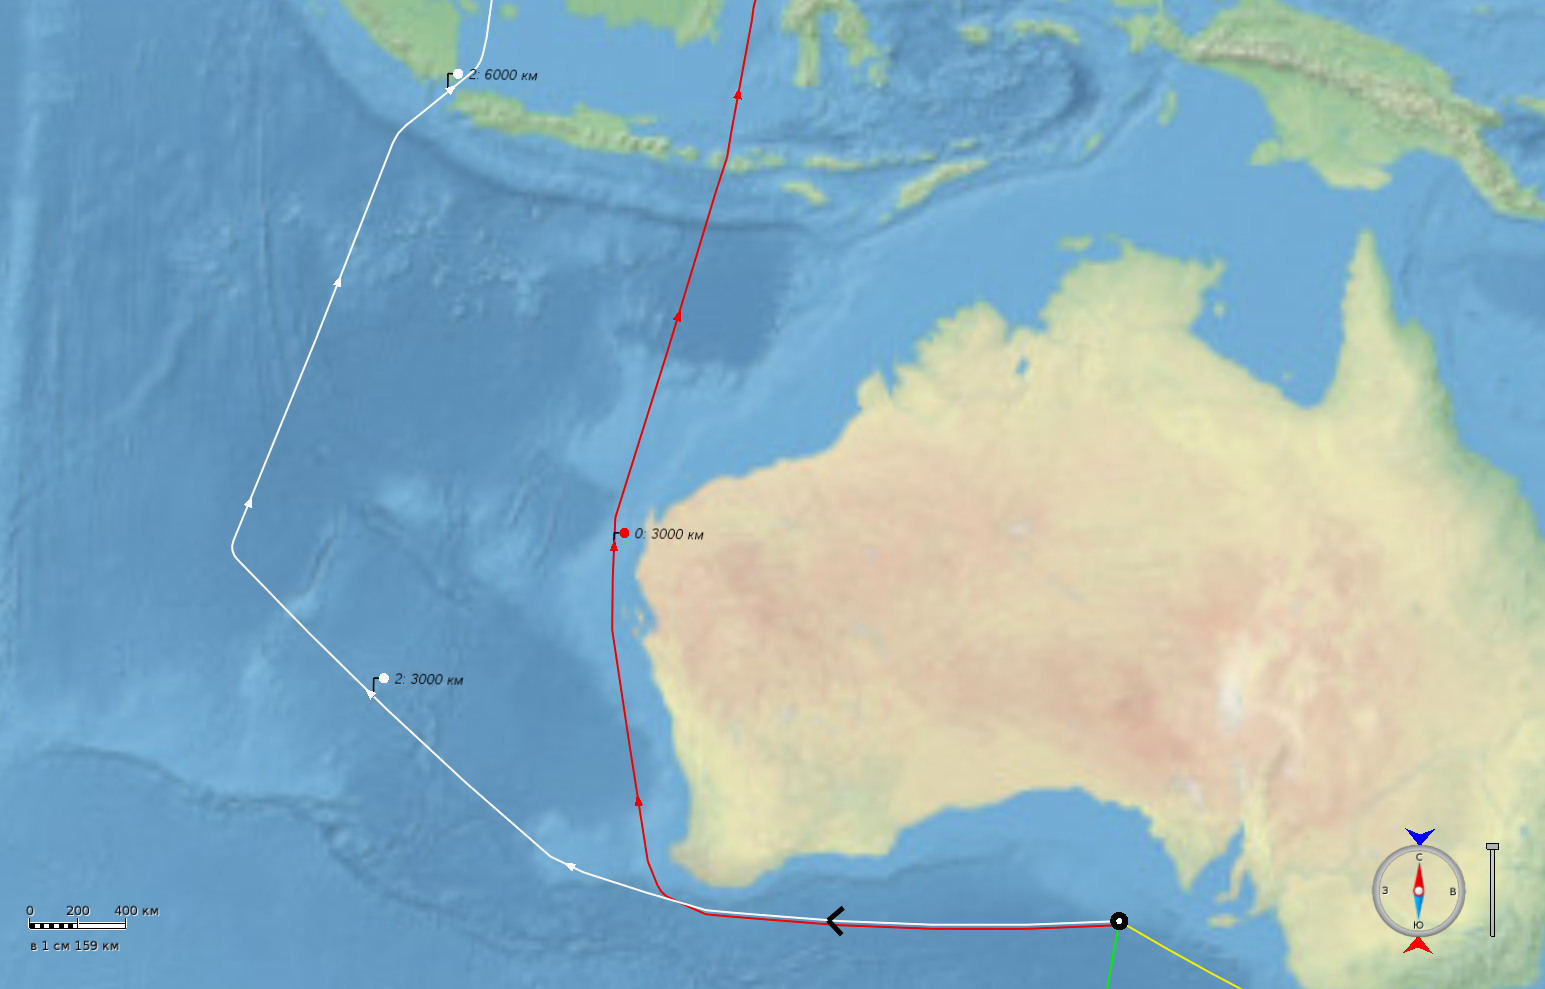
\includegraphics[clip=true, trim = 300pt 20pt 330pt 350pt, width=\textwidth]{Solution/weights-on-path-good}
          \end{columns}

            На маршруте потенциалы меньше, чем поблизости
        \end{figure}
    }
\end{frame}
\note {
Это тут пока просто так.

1. Рассмотрим такую ситуацию, вершины находятся довольно близко,
поэтому их потенциалы примерно равны какому-то C. При этом, если
прибавлять среднее арифметическое, то стоимость верхнего пути
получится на C больше, хотя он лучше. Поэтому будем домножать на
среднее геометрическое. В таком случае вклад потенциалов будет
примерно равен, и будет найден верхний маршрут.

2. Слева показана ситуация, где потенциалы аккумулируются, а справа —
где берётся максимум. Во первом случае почти весь вклад потенциалов
сосредоточен в начале и конце. И в результате эксперимента во втором
случае оказалось найдено на один маршрут больше.

3. Если потенциал монотонно убывает с ростом кратчайшего расстояния от
найденнного маршрута, то на маршруте будут самые большие потенциалы,
поэтому следующий маршрут может отличаться в местах, где он ожидается
таким же. Для получения более естественного результата немного
уменьшим потенциалы вершин маршрута.
}

\end{document}

